\chapter{Schéma à pas de temps local}
\label{chap:pas de temps local}

Dans le chapitre précédent, nous avons décrit l'implémentation
de la version parallèle du solveur, pouvant utiliser simultanément
un grand nombre d'accélérateurs.
Cette capacité de gérer plusieurs accélérateurs nous a déjà
permis d'accélérer considérablement la vitesse de calcul.

Afin d'améliorer encore la vitesse de calcul du solveur, sans avoir recours
à de plus puissants et plus nombreux accélérateurs, nous allons présenter une
adaptation algorithmique très efficace.
Après avoir détaillé les schémas temporels de type Runge-Kutta
dans la section \ref{sect:schemas_temporels}, nous allons 
à présent décrire un schéma inspiré des méthodes de type ADER initialement proposée
par Toro (voir par exemple \cite{schwartzkopff2002ader,schwartzkopff2004fast}).
\\

Le schéma LRK$2$ (pour « \textit{Local} RK$2$ ») que nous présentons dans cette section est une adaptation du
schéma RK$2$, modifié à l'aide d'une phase de prédiction locale. Le shéma RK$2$ tel que présenté
dans la partie \ref{ssect:rk} se décompose en $2$ étapes faisant chacune intervenir
l'opérateur $\mathcal{G}$ qui permet d'évaluer la dérivée à un instant $t$ donné
par la méthode Galerkin Discontinue (GD).
Le schéma LRK$2$ reprend les mêmes
étapes que le schéma RK$2$ à la différence près que l'opérateur $\mathcal{G}$ de la première
étape est remplacé par une version locale de celui-ci.

Nous utilisons ensuite les propriétés locales du schéma LRK$2$ afin
de découpler l'avancée en temps de l'approximation de la solution sur
les différentes mailles. Ce second schéma, que nous appellerons
LTS$2$ (pour « \textit{Local Time Step} $2$ »), permettra alors de réduire
considérablement le temps de simulation en divisant la quantité
de calculs lorsque la géométrie est composée de mailles de tailles très hétérogènes.
\\

\section{Approximation locale en dimension 1}
\label{sect:pas de temps local dim 1}

\begin{remark}
	Nous décrivons les modifications apportées à la méthode GD
	\eqref{eq:formulation_semi-discrete} en dimension $1$ d'espace %\todo{mettre "dimension un" partout}.
	Il s'agit de l'implémentation développée afin de tester
	la méthode sur un cas simple d'équation du transport.
	Ces modifications se généralisent facilement en dimension $3$.
\end{remark}

Nous considérons le problème d'évolution \eqref{eq:probleme_evolution}
pour un système de Friedrichs \eqref{eq:friedrichs}.
Afin de simplifier les écritures, nous considérons le problème
sans sources ($\ACnd = 0$ et $\Src = 0$) et nous supposons
que la matrice $\At$ est égale à l’identité.
Dans ces conditions, le problème d'évolution s'écrit :
\begin{align}
	\Ptl{t} \W + \A \Ptl{\x} \W = 0 .
\end{align}



\subsection{Formulation GD en dimension 1}
\label{ssect:formulation_gd_1-d}


Nous considérons le maillage $\Mesh$ du domaine
$\PbEsp = \ItvOO{a}{b}$ donné par l'ensemble des points
$(\Nd{i})_{i \in \Range{0}{\NE}}$ tels que :
\begin{align}
	a = \Nd{0} < \ldots < \Nd{\NE} = b .
\end{align}
Les mailles $(\L_i)_{i \in \Range{1}{\NE}}$ sont donc
les intervalles :
\begin{align}
	\L_i = \ItvOO{\Nd{i - 1}}{\Nd{i}} ,
	\; \mathrm{pour} \; i \in \Range{1}{\NE} .
\end{align}

\begin{remark}
	Puisque nous décrivons cette méthode en dimension $1$, dans la suite,
	nous notons $\L$ l'indice de la maille $\L_i$ considérée.
	Les indices des mailles voisines, $\L_{i + j}$ pour
	$j \in \EnsZ^\star$, sont alors notés $\L + j$. 
\end{remark}


Nous utilisons alors l'élément de référence $\hat{\L} = \ItvOO{0}{1}$.
Dans chaque maille, nous considérons une approximation spatiale
d'ordre $\Deg$, avec $\Deg + 1$ points d'approximation par maille.
Les points $(\GLN{i})_{i \in \RangeDeg}$ et poids
$(\GLW{i})_{i \in \RangeDeg}$ d'interpolation choisis sont
ceux de Gauss-Lobatto.
\begin{remark}
	Nous aurions pu utiliser une interpolation à l'aide des points de
	Gauss-Legendre d'ordre $\Deg$. L'utilisation des points
	de Gauss-Lobatto, par la présence des points de bord, simplifie
	l'implémentation en supprimant l'extrapolation des champs sur les
	interfaces entre les mailles.
\end{remark}
Les fonctions de base sur l'élément de référence $\hat{\L}$ sont données
par les polynômes de Lagrange d'ordre $\Deg$ définis par :
\begin{align}
	\PsiRef{i}(\xref) = \prod_{\substack{j=0 \\ j \neq i}}^{\Deg}
	\frac{\xref - \GLN{j}}{\GLN{i} - \GLN{j}} ,
	\; \mathrm{pour} \; i \in \RangeDeg ,
\end{align}
ainsi, par définition :
\begin{align}
	\PsiRef{i}(\GLN{j}) = \delta_{i,j} .
\end{align}

Nous notons $\TGeo{\L}$ la transformation permettant de passer
de l'élément de référence $\hat{\L}$ à la maille physique
$\L = \ItvOO{\Nd{\L - 1}}{\Nd{\L}}$.
L'expression de celle-ci est donnée par :
\begin{align}
	\TGeo{\L}(\xref) = \Nd{\L - 1} + 
	\xref (\Nd{\L} - \Nd{\L - 1}) .
\end{align}
Pour une maille $\L$ donnée (figure \ref{img:ader_1d_mesh}),
les points d'approximation physiques sont notés :
\begin{align}
	\GLNPhy{\L}{i} = \TGeo{\L}(\GLN{i}),
	\; \mathrm{pour} \; i \in \RangeDeg ,
\end{align}
et les fonctions de base physiques sont données par :
\begin{align}
	\PsiPhy{\L}{i} \circ \TGeo{\L}(\xref) = \PsiRef{i}(\xref)
	\Leftrightarrow
	\PsiPhy{\L}{i} (\x) = \PsiRef{i} \circ \Inv{\TGeo{\L}} (\x) .
\end{align}
Ainsi, dans chaque maille $\L$, nous approchons $\W(\x,t)$ par :
\begin{align}
	\W(\x,t) 
	\approx \sum_{i=0}^{\Deg} \W_{\L,i}(t) \PsiPhy{\L}{i}(\x)
	= \W_{\L,i}(t) \PsiPhy{\L}{i}(\x)
	\label{eq:ader_approx_w} ,
\end{align}
en utilisant la convention de sommation des indices répétés.


\begin{figure}[h]
	\begin{center}
		\caption{
			\label{img:ader_1d_mesh}
			Mailles et points d'approximations du maillage considéré
			pour l'ordre d'approximation $3$.
		}

		\tikzstyle{brace}=[
			decoration={brace, raise = 0.2em}, decorate
		]
		
		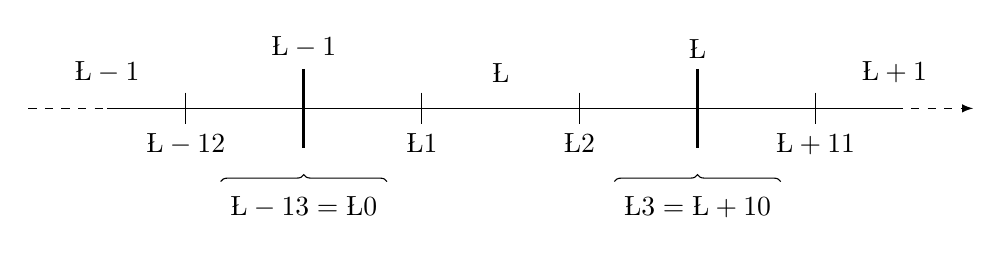
\begin{tikzpicture}[scale=1]
			% axe
			\draw[dashed] (0,0) -- (1,0);
			\draw[-] (1,0) -- (11,0);
			\draw[dashed,arrows={-latex}] (11,0) -- (12,0);
			
			% noeuds
			\draw[-,very thick] (3.5,0.5) node[above] {$\Nd{\L-1}$} -- (3.5,-0.5);
			\draw[-,very thick] (8.5,0.5) node[above] {$\Nd{\L}$} -- (8.5,-0.5);
			
			% mailles
			\draw (1,0.2) node[above] {$\L-1$};
			\draw (6,0.2) node[above] {$\L$};
			\draw (11,0.2) node[above] {$\L+1$};

			% points approx
			\draw[-] (2,0.2) -- (2,-0.2) node[below] {$\GLNPhy{\L-1}{2}$};
			\draw (3.5,-1) node (nd1) [below] {$\GLNPhy{\L-1}{3} = \GLNPhy{\L}{0}$};
			\draw[brace] (nd1.north west) -- (nd1.north east);
			\draw[-] (5,0.2) -- (5,-0.2) node[below] {$\GLNPhy{\L}{1}$};
			\draw[-] (7,0.2) -- (7,-0.2) node[below] {$\GLNPhy{\L}{2}$};
			\draw (8.5,-1) node (nd2) [below] {$\GLNPhy{\L}{3} = \GLNPhy{\L+1}{0}$};
			\draw[brace] (nd2.north west) -- (nd2.north east);
			\draw[-] (10,0.2) -- (10,-0.2) node[below] {$\GLNPhy{\L+1}{1}$};
			
		\end{tikzpicture}
	\end{center}
\end{figure}



Avec ces notations, nous avons la formulation GD suivante : 
trouver une solution $\W$ telle que :
\begin{equation}
	\begin{aligned}
	\forall \L = \ItvOO{\Nd{\L - 1}}{\Nd{\L}} &\in \Mesh ,
	\forall \PsiPhy{\L}{i} \in \mathcal{C}^1(\Adh{\L}), \\
		\int_{\L} \Ptl{t} \W \PsiPhy{\L}{i} d\x
		&- \int_{\L} \A \W \Ptl{\x} \PsiPhy{\L}{i} d\x \\
		&+ (\Pos{\A} \W(\Neg{\Nd{\L}},t) +
			\Neg{\A} \W(\Pos{\Nd{\L}},t))
			\PsiPhy{\L}{i} (\Neg{\Nd{\L}}) \\
		&- (\Neg{\A} \W(\Pos{\Nd{\L - 1}},t) +
			\Pos{\A} \W(\Neg{\Nd{\L - 1}},t))
			\PsiPhy{\L}{i} (\Pos{\Nd{\L - 1}}) = 0 ,
	\end{aligned}
\end{equation}
où $\Pos{\A}$, respectivement $\Neg{\A}$, représente
la partie positive, respectivement négative, de $\A$
(définition \ref{def:matrix_pos_neg})
et $\W(\Pos{\Nd{\L}},t)$, respectivement $\W(\Neg{\Nd{\L}},t)$, représente
la valeur de $\W$ à l'instant $t$ en $\Nd{\L}$ à droite,
respectivement à gauche.
En d'autres termes :
\begin{subequations}
	\begin{align}
		\W(\Pos{\Nd{\L}},t) &=
		\lim\limits_{\substack{\varepsilon \rightarrow 0 \\ \varepsilon > 0}}
		\W(\Nd{\L} + \varepsilon,t) = \W_{\L+1,0}(t) , \\
		\W(\Neg{\Nd{\L}},t) &=
		\lim\limits_{\substack{\varepsilon \rightarrow 0 \\ \varepsilon > 0}}
		\W(\Nd{\L} - \varepsilon,t) = \W_{\L,\Deg}(t) .
	\end{align} 
\end{subequations}
Et de même pour l'évaluation de la fonction $\PsiPhy{\L}{i}$ :
\begin{subequations}
	\begin{align}
		\PsiPhy{\L}{i} (\Pos{\Nd{\L-1}}) &=
		\lim\limits_{\substack{\varepsilon \rightarrow 0 \\ \varepsilon > 0}}
		\PsiPhy{\L}{i} (\Nd{\L-1} + \varepsilon) =
		\PsiPhy{\L}{i} (\GLNPhy{\L}{0}) = \delta_{i,0} , \\
		\PsiPhy{\L}{i} (\Neg{\Nd{\L}}) &=
		\lim\limits_{\substack{\varepsilon \rightarrow 0 \\ \varepsilon > 0}}
		\PsiPhy{\L}{i}(\Nd{\L} - \varepsilon) =
		\PsiPhy{\L}{i} (\GLNPhy{\L}{\Deg}) = \delta_{i,\Deg} .
	\end{align} 
\end{subequations}

En utilisant l'approximation de $\W$ dans la base d'approximation
\eqref{eq:ader_approx_w}, nous obtenons :
\begin{equation}
	\begin{aligned}
		\int_{\L} \Ptl{t} \W_{\L,j} \PsiPhy{\L}{j} \PsiPhy{\L}{i} d\x
		&- \int_{\L} \A \W_{\L,j} \PsiPhy{\L}{j} \Ptl{\x} \PsiPhy{\L}{i} d\x \\
		&+ (\Pos{\A} \W_{\L,\Deg} +
		\Neg{\A} \W_{\L+1,0}) \delta_{i,\Deg}  \\
		&- (\Neg{\A} \W_{\L,0} +
		\Pos{\A} \W_{\L-1,\Deg}) \delta_{i,0} = 0
		\label{eq:ader_pb} .
	\end{aligned}
\end{equation}
%\todo{la matrice masse est diagonale. Simplifier cette expression}
Ainsi, en supposant connue la solution à l'instant $t = \alpha$, nous pouvons
évaluer la solution à l'instant $t = \beta > \alpha$ en intégrant
\eqref{eq:ader_pb} sur $\ItvCC{\alpha}{\beta}$ :
\begin{equation}
	\begin{aligned}
		\left( \int_{\L} \PsiPhy{\L}{j} \PsiPhy{\L}{i} d\x \right)
		&\left( \W_{\L,j}(\beta) - \W_{\L,j}(\alpha) \right) \\
		&- \int_{t=\alpha}^{\beta} \int_{\L} \A \W_{\L,j} \PsiPhy{\L}{j} \Ptl{\x} \PsiPhy{\L}{i} d\x dt \\
		&+ \int_{t=\alpha}^{\beta} (\Pos{\A} \W_{\L,\Deg} +
		\Neg{\A} \W_{\L+1,0}) \delta_{i,\Deg} dt \\
		&- \int_{t=\alpha}^{\beta} (\Neg{\A} \W_{\L,0} +
		\Pos{\A} \W_{\L-1,\Deg}) \delta_{i,0} dt = 0
		\label{eq:ader_pb_int_t} .
	\end{aligned}
\end{equation}
En appliquant les simplifications vues dans la section
\ref{ssect:terme_de_masse}, le terme de masse devient :
\begin{align}
	\int_{\L} \PsiPhy{\L}{j} \PsiPhy{\L}{i} d\x
	= \GLW{i} (\Nd{\L} - \Nd{\L - 1}) .
\end{align}

Nous allons nous placer dans un cadre un peu plus général. Nous pouvons aussi considérer
 un système d'équations différentielles
ordinaires défini par un graphe $G=(\Mesh,E)$, où l'ensemble des nœuds du graphe est noté $\Mesh$ 
et $E \subset \Mesh^2$ est l'ensemble des arêtes orientées du graphe. Dans notre cas $\Mesh$ est 
l'ensemble des mailles $\L$ du maillage et $E$ s'identifie à l'ensemble des interfaces entre deux mailles
voisines.
Avec ces notations, l'équation différentielle \eqref{eq:ader_pb} s'écrit pour chaque nœud du
$\L$ graphe :
\begin{align} \label{eq:ader_sys_gd}
	\Ptl{t} \W_\L = \sum_{(\L,\R) \in E}
		\bm{\mu}_{\L,\R} (\W_\L, \W_\R) ,
\end{align}
où les $\bm{\mu}_{\L,\R}$ sont des matrices de couplage entre les inconnues des mailles $\L$ et $\R$.
L'expression de la solution au temps $t = \beta$ en fonction
de la solution connue au temps $t = \alpha$ devient alors :
\begin{align}
	\W_\L(\beta) - \W_\L(\alpha) =
	\int_{t=\alpha}^{\beta} \sum_{(\L,\R) \in E}
	\bm{\mu}_{\L,\R} (\W_\L, \W_\R)
	\label{eq:ader_sys_gd_int_t} .
\end{align}


Remarquons que le système composé des équations \eqref{eq:ader_sys_gd}
permet de déterminer la dérivée en temps
de la solution à un instant donné pour lequel la solution est connue.
Cette opération correspond à l'application de l'opérateur $\mathcal{G}$
\eqref{eq:operateur_gd} en dimension $1$.
\\


\subsection{Formulation GD locale en dimension 1}
\label{ssect:formulation_gd_locale}


Afin de supprimer le couplage entre les mailles,
nous approchons l'équation différentielle
\eqref{eq:ader_pb} par un « prédicteur » local
à la maille :
\begin{equation}
	\begin{aligned}
		\int_{\L} \Ptl{t} \V_{\L,j} \PsiPhy{\L}{j} \PsiPhy{\L}{i} d\x
		&- \int_{\L} \A \V_{\L,j} \PsiPhy{\L}{j} \Ptl{\x} \PsiPhy{\L}{i} d\x \\
		&+ (\Pos{\A} \V_{\L,\Deg} +
		\Neg{\A} \V_{\L,\Deg}) \delta_{i,\Deg} \\
		&- (\Neg{\A} \V_{\L,0} +
		\Pos{\A} \V_{\L,0}) \delta_{i,0} = 0 .
	\end{aligned}
\end{equation}
Puis, en simplifiant les termes de bord :
\begin{equation}
\begin{aligned}
\int_{\L} \Ptl{t} \V_{\L,j} \PsiPhy{\L}{j} \PsiPhy{\L}{i} d\x
&- \int_{\L} \A \V_{\L,j} \PsiPhy{\L}{j} \Ptl{\x} \PsiPhy{\L}{i} d\x \\
&+ \A (\V_{\L,\Deg} \delta_{i,\Deg}
- \V_{\L,0} \delta_{i,0}) = 0 .
\end{aligned}
\end{equation}
Nous obtenons ainsi un autre système d'équations différentielles dont
la solution est une approximation locale du problème \eqref{eq:ader_pb} ou \eqref{eq:ader_sys_gd},
$\V_\L \approx \W_\L$. Dans notre formalisme d'équations différentielles
posées sur les nœuds d'un graphe, \eqref{eq:ader_sys_gd} est donc approché par un système diagonal, sans interaction 
entre les nœuds voisins. Ce système diagonal est de la forme
\begin{align} \label{eq:ader_sys_gd_local}
	\Ptl{t} \V_\L = \bm{\nu}_{\L} (\V_\L) ,
\end{align}
où les termes de couplage $\bm{\mu}_{\L,\R}$ sont remplacés par une approximation diagonale $\bm{\nu}_{\L}$.
Nous notons $\mathcal{G}_l$ l'opérateur associé à l'évaluation
de la dérivée en temps à l'aide du système composé
des équations \eqref{eq:ader_sys_gd_local}.

Nous sommes alors en mesure de calculer une prédiction locale de la dérivée
en temps à partir de la solution de bonne qualité $\W$, à l'aide
du système \eqref{eq:ader_sys_gd_local} :
\begin{align}
	\Ptl{t} \V = \mathcal{G}_l (\W, t)
	\label{eq:operateur_gd_local} .
\end{align}

\begin{remark}
	L'application de l'opérateur $\mathcal{G}_l$ correspond à l'application
	de l'opérateur $\mathcal{G}$ \eqref{eq:operateur_gd} en remplaçant
	le flux d'interface $\Flux{\W_\L}{\W_\R}{\n}$ par le flux
	local $\Flux{\W_\L}{\W_\L}{\n}$.
\end{remark}

\begin{remark}
	Ce prédicteur ne prend pas en compte la valeur de la solution
	des mailles voisines. L'évaluation de la dérivée en temps ne doit donc
	pas être calculée uniquement à l'aide de cet opérateur.
	Nous l'utilisons, comme son nom l'indique, dans la phase de
	prédiction, une mise-à-jour étant toujours calculée à l'aide
	du système d'approximation GD \eqref{eq:ader_sys_gd}.
	\\
	En appliquant la prédiction locale \eqref{eq:ader_sys_gd_local},
	nous admettons que les variables conservatives à gauche et à droite
	des interfaces entre les mailles sont identiques.
	Nous négligeons alors cet écart afin de réduire les coûts de calcul
	et, dans la suite, découpler l'avancée en temps des mailles.
\end{remark}



Supposons calculée la solution $\W$ au temps $t = \alpha$. Pour calculer
la solution au temps $t = \beta$, nous utilisons alors la mise-à-jour :
\begin{align}
	\W_\L(\beta) - \W_\L(\alpha) =
	\int_{t=\alpha}^{\beta} \sum_{(\L,\R) \in E}
		\bm{\mu}_{\L,\R} (\V_\L, \V_\R)
	\label{eq:methode_locale_int_t_cont} ,
\end{align}
où $\V$ est calculé grâce au équations différentielles locales \eqref{eq:ader_sys_gd_local}.
Cette intégrale en temps peut être approchée par n'importe quelle formule
de quadrature, par exemple la méthode du point milieu :
\begin{align}
	\begin{aligned}
		\W_\L(\beta) &- \W_\L(\alpha) \approx \\ 
		&(\beta - \alpha) \sum_{(\L,\R) \in E}
			\bm{\mu}_{\L,\R} &\left(\V_\L \left(\frac{\alpha + \beta}{2}\right),
				\V_\R \left(\frac{\alpha + \beta}{2}\right)\right)
		\label{eq:methode_locale_int_t_pm} .
	\end{aligned}
\end{align}
Il s'agit là du schéma LRK$2$ que nous présentons ci-après
(voir \ref{sect:pas de temps local lrk2}).

De manière plus générale, nous pouvons choisir une intégration temporelle
propre à chaque maille, à l'aide de points de Gauss temporels.
Afin d'avancer la solution en temps sur une maille donnée,
une prédiction doit être calculée en chaque point temporel,
sur la maille considérée ainsi que sur ses voisins.
La mise-à-jour s'effectue ensuite en appliquant la formule de quadrature
temporelle \eqref{eq:methode_locale_int_t_cont} avec ces prédictions.
\\


\section{Schéma LRK2}
\label{sect:pas de temps local lrk2}


L'avancée en temps dans l'évaluation de la solution peut se faire
sur le modèle du schéma RK$2$ \eqref{eq:methode_rk2}, en substituant la première étape
par une prédiction locale \eqref{eq:operateur_gd_local} :
\begin{equation}
	\begin{aligned}
		\V^{n+\frac{1}{2}} &= \W^n
		+ \frac{\dt}{2} \mathcal{G}_l(\W^n,t) , \\
		\W^{n+1} &= \W^n
		+ \dt \mathcal{G}\left(\V^{n+\frac{1}{2}},t + \frac{\dt}{2}\right)
		\label{eq:methode_lrk2} .
	\end{aligned}
\end{equation}
Il s'agit de la formule d'intégration temporelle
\eqref{eq:methode_locale_int_t_pm}
appliquée de manière uniforme sur tout le maillage.
Là aussi, la première étape est appelée prédiction
et la seconde étape est appelée mise-à-jour.
Le graphe des tâches de l'étape de prédiction locale
du schéma couplé GD-LRK$2$ est donné dans la figure \ref{img:graphe_lrk2}.
L'étape de mise-à-jour est identique à celle du schéma couplé GD-RK$2$
dont le graphe des tâches est présenté dans la figure \ref{img:graphe_rk2}.

La stabilité et la convergence de cette méthode sont expérimentalement
démontrées équivalentes au schéma RK$2$ dans les sections
\ref{sect:pas de temps local transport} (équation du transport $1$-d)
et \ref{ssect:tete_simplifiee_lrk2} (équations de Maxwell $3$-d).
De plus, un facteur d'accélération
non négligeable a été constaté suite à la simplification des
flux d'interfaces entre les mailles. Nous présentons ces résultats
dans la section~\ref{ssect:tete_simplifiee_lrk2}.
\\


\begin{figure}[!h]
	\centering
	\caption{
		\label{img:graphe_lrk2}
		Graphe des tâches du demi pas de temps de prédiction locale
		du schéma couplé GD-LRK$2$ pour deux zones homogènes.
		L'étape de mise-à-jour est donnée dans la figure \ref{img:graphe_rk2}.
	}
	\begin{tikzpicture}[scale=1]
	\node[ellipse,very thick,draw,align=center] (debut)
	at (0,-4) {Début du demi\\pas de temps\\de prédiction};
	
	\node[ellipse,very thick,draw=blue,fill=blue!10,align=center] (volume1)
	at (-4,-6) {Zone 1\\Terme de volume};
	\node[ellipse,very thick,draw=red,fill=red!10,align=center] (flux1)
	at (-3.5,-8) {Zone 1\\Terme de flux \textbf{local}};
	\node[ellipse,very thick,draw=green,fill=green!10,align=center] (masse1)
	at (-3,-10) {Zone 1\\Terme de masse};
	\node[ellipse,very thick,draw=gray,fill=gray!10,align=center] (euler1)
	at (-2.5,-12) {Zone 1\\Etape d'Euler};
	
	\node[ellipse,very thick,draw=blue,fill=blue!10,align=center] (volume2)
	at (4,-6) {Zone 2\\Terme de volume};
	\node[ellipse,very thick,draw=red,fill=red!10,align=center] (flux2)
	at (3.5,-8) {Zone 2\\Terme de flux \textbf{local}};
	\node[ellipse,very thick,draw=green,fill=green!10,align=center] (masse2)
	at (3,-10) {Zone 2\\Terme de masse};
	\node[ellipse,very thick,draw=gray,fill=gray!10,align=center] (euler2)
	at (2.5,-12) {Zone 2\\Etape d'Euler};
	
	\node[ellipse,very thick,draw,align=center] (fin)
	at (0,-14) {Fin du demi\\pas de temps\\de prédiction};
	
	\path[arrows={-latex},very thick] (debut) edge[out=180,in=90] (volume1);
	\path[arrows={-latex},very thick] (debut) edge[out=0,in=90] (volume2);
	\path[arrows={-latex},very thick] (volume1) edge (flux1);
	\path[arrows={-latex},very thick] (volume2) edge (flux2);
	\path[arrows={-latex},very thick] (flux1) edge (masse1);
	\path[arrows={-latex},very thick] (flux2) edge (masse2);
	\path[arrows={-latex},very thick] (masse1) edge (euler1);
	\path[arrows={-latex},very thick] (masse2) edge (euler2);
	\path[arrows={-latex},very thick] (euler1) edge (fin);
	\path[arrows={-latex},very thick] (euler2) edge (fin);
	\end{tikzpicture}
\end{figure}




\section{Schéma LTS2}
\label{sect:pas de temps local}


Les critères de stabilité de type CFL donnent des pas de temps 
proportionnels à la taille des mailles. Or, dans le cas
des schémas que nous avons présenté précédemment, l'avancée en temps
de la solution s'effectue au rythme du plus petit pas de temps.
Ainsi, dans le cas de maillages contenant des mailles de tailles très
variées, une méthode permettant de faire avancer la solution sur
chaque maille au rythme du pas de temps propre à cette maille
nous donnerait un important facteur d'accélération en réduisant
la quantité de calculs nécessaires.

C'est le cas du schéma que nous présentons ici.
Nous utilisons les propriétés locales du prédicteur $\mathcal{G}_l$
afin de découpler l'avancée en temps de la solution sur les mailles.
Rappelons que cet opérateur permet d'estimer la valeur de la solution
à un instant donné, indépendamment des mailles voisines.


\subsection{Description}
\label{ssect:lts2_desc}

\begin{remark}
	Nous nous replaçons dans le cas en dimension $1$ pour les explications
	schématiques de cette métode.
\end{remark}


Considérons les mailles $\L$, $\L+1$, $\L+2$
et $\dt_\L$, $\dt_{\L+1}$, $\dt_{\L+2}$ leurs pas
de temps respectifs donnés par l'application d'un critère CFL de stabilité.
Supposons ces mailles définies telles que :
\begin{align}
	\dt_{\L+2} \ge \dt_{\L+1} = 2 \dt_\L .
\end{align}

Avec un schéma temporel à pas de temps uniforme tel que les schémas
de type RK, la solution sur toutes ces mailles
avance d'un pas de temps $\dt_\L$ à chaque itération.
En effet, ce pas de temps est imposé par la maille $\L$
qui nécessite l'avancée synchronisée de la maille $\L+1$
afin de procéder de manière consistante et conservative au calcul
du flux entre les mailles (figure~\ref{img:ader_flux_rk}).
Ainsi, de proche en proche, la solution évolue sur le maillage complet
avec le plus petit pas de temps à chaque itération.

Dans les figures \ref{img:ader_flux_rk},
\ref{img:ader_flux_lrk} et \ref{img:ader_flux_lrk_ldt},
les lignes pointillées rouges représentent le
domaine de définition de la solution aux différentes étapes
des schémas d'intégration temporelle présentés.
La solution peut être définie à chaque étape sur le maillage complet
(figures \ref{img:ader_flux_rk} et \ref{img:ader_flux_lrk})
ou partiellement sur quelques mailles (figure \ref{img:ader_flux_lrk_ldt}).
Afin d'avancer en temps (passer d'une ligne pointillée rouge à la suivante),
nous appliquons l'opérateur $\mathcal{G}$ ou l'opérateur $\mathcal{G}_l$
suivi d'une étape de type Euler (section \ref{ssect:etape_euler}).
Seul le terme de flux (local ou non) des opérateurs est réprésenté
dans ces figures à l'aide de flèches.


\begin{remark}
	Dans la suite, nous utiliserons l'abus de notation qui consiste
	à identifier une maille à sa solution. Ainsi, lorsque nous dirons
	qu'une maille avance d'un pas de temps $\dt$, cela signifie que
	la solution définie sur cette maille est avancée d'un pas de
	temps $\dt$ par une méthode d'intégration, ou de manière
	plus générale, par un schéma temporel.
\end{remark}

\newcommand{\AderShemeScales}{1}
\begin{figure}[!h]
	\begin{center}
		\caption{
			\label{img:ader_flux_rk}
			Calcul d'un pas de temps RK$2$ dans une configuration
			de mailles hétérogènes. Les étapes dans le calcul de la
			solution sont en pointillés rouges. Le calcul des flux
			dans l'opérateur $\mathcal{G}$
			est représenté par les cercles bleus et leur application
			via l'avancée en temps par les flèches bleues.
		}
		
		\tikzstyle{fluxarrow}=[-,blue,arrows={-latex},thick,shorten <=5pt,shorten >=2pt]
		
		\tikzstyle{fluxcircle}=[blue,thick]
		
		\begin{tikzpicture}[scale=\AderShemeScales]
		% rectangles gris
		\draw[fill=gray!10] (0,0) rectangle (2,2);
		\draw[fill=gray!10] (2,0) rectangle (6,4);
		\draw[fill=gray!10] (6,0) rectangle (10,4);

		% axe x
		\draw[-,arrows={-latex}] (0,0) -- (11,0) node[below right] {$\PbEsp$};
		
		% axe t
		\draw[-,arrows={-latex}] (0,0) -- (0,5) node[above left] {$t$};
		
		% noeuds
		\draw[-] (0,-0.1) -- (0,2) -- (2,2);
		\draw[-] (2,-0.1) -- (2,4) -- (6,4);
		\draw[-] (6,-0.1) -- (6,4) -- (10,4);
		\draw[-] (10,-0.1) -- (10,4);
		
		% mailles
		\draw (1,-0.2) node[below] {$\L$};
		\draw (4,-0.2) node[below] {$\L+1$};
		\draw (8,-0.2) node[below] {$\L+2$};
		
		% dt
		\draw[-] (-0.1,2) node[below left] {$\dt_\L$} -- (0.1,2);
		\draw[-] (-0.1,4) node[left] {$2 \dt_\L$} -- (0.1,4);
		\draw[dotted] (0.1,4) -- (2,4);
		
		% solutions
		\draw[dashed,red,very thick] (0,0) node[left] {$\W^n$} -- (10,0);
		\draw[dashed,red,very thick] (0,1) node[left] {$\W^{n+\frac{1}{2}}$} -- (10,1);
		\draw[dashed,red,very thick] (0,2) node[above left] {$\W^{n+1}$} -- (10,2);
		
		% flux
		\draw[fluxcircle] (0,0) circle (0.15);
		\draw[fluxcircle] (2,0) circle (0.15);
		\draw[fluxcircle] (6,0) circle (0.15);
		\draw[fluxcircle] (10,0) circle (0.15);
		\draw[fluxcircle] (0,1) circle (0.15);
		\draw[fluxcircle] (2,1) circle (0.15);
		\draw[fluxcircle] (6,1) circle (0.15);
		\draw[fluxcircle] (10,1) circle (0.15);

		% application
		\draw[fluxarrow] (0,0) -- (1,1);
		\draw[fluxarrow] (2,0) -- (1,1);
		\draw[fluxarrow] (2,0) -- (3,1);
		\draw[fluxarrow] (6,0) -- (5,1);
		\draw[fluxarrow] (6,0) -- (7,1);
		\draw[fluxarrow] (10,0) -- (9,1);
		
		\draw[fluxarrow] (0,1) -- (1,2);
		\draw[fluxarrow] (2,1) -- (1,2);
		\draw[fluxarrow] (2,1) -- (3,2);
		\draw[fluxarrow] (6,1) -- (5,2);
		\draw[fluxarrow] (6,1) -- (7,2);
		\draw[fluxarrow] (10,1) -- (9,2);

		\end{tikzpicture}
	\end{center}
\end{figure}

Dans le cas du schéma LRK$2$ \eqref{eq:methode_lrk2}, l'avancée en temps
doit aussi s'effectuer de manière synchronisée (figure \ref{img:ader_flux_lrk})
au rythme du plus petit pas de temps.
%\todo{mieux expliquer à quoi
%	correspondent les pointillés rouges}

\begin{figure}[!h]
	\begin{center}
		\caption{
			\label{img:ader_flux_lrk}
			Calcul d'un pas de temps LRK$2$ dans une configuration
			de mailles hétérogènes. Les étapes dans le calcul de la
			solution sont en pointillés rouges. Le calcul des flux
			dans l'opérateur $\mathcal{G}$
			est représenté par les cercles bleus et leur application
			via l'avancée en temps par les flèches bleues.
			Le calcul des flux locaux
			dans l'opérateur $\mathcal{G}_l$
			est représenté par les demi-disques verts et leur application
			via l'avancée en temps par les flèches vertes.
		}
		
		\tikzstyle{fluxarrow}=[-,blue,arrows={-latex},thick,shorten <=5pt,shorten >=2pt]
		
		\tikzstyle{fluxcircle}=[blue,thick]
		
		\tikzstyle{lfluxarrow}=[-,green,arrows={-latex},thick,shorten <=5pt,shorten >=2pt]
		
		\tikzstyle{lfluxcircle}=[green,thick]

		\begin{tikzpicture}[scale=\AderShemeScales]
		% rectangles gris
		\draw[fill=gray!10] (0,0) rectangle (2,2);
		\draw[fill=gray!10] (2,0) rectangle (6,4);
		\draw[fill=gray!10] (6,0) rectangle (10,4);
		
		% axe x
		\draw[-,arrows={-latex}] (0,0) -- (11,0) node[below right] {$\PbEsp$};
		
		% axe t
		\draw[-,arrows={-latex}] (0,0) -- (0,5) node[above left] {$t$};
		
		% noeuds
		\draw[-] (0,-0.1) -- (0,2) -- (2,2);
		\draw[-] (2,-0.1) -- (2,4) -- (6,4);
		\draw[-] (6,-0.1) -- (6,4) -- (10,4);
		\draw[-] (10,-0.1) -- (10,4);
		
		% mailles
		\draw (1,-0.2) node[below] {$\L$};
		\draw (4,-0.2) node[below] {$\L+1$};
		\draw (8,-0.2) node[below] {$\L+2$};
		
		% dt
		\draw[-] (-0.1,2) node[below left] {$\dt_\L$} -- (0.1,2);
		\draw[-] (-0.1,4) node[left] {$2 \dt_\L$} -- (0.1,4);
		\draw[dotted] (0.1,4) -- (2,4);
		
		% solutions
		\draw[dashed,red,very thick] (0,0) node[left] {$\W^n$} -- (10,0);
		\draw[dashed,red,very thick] (0,1) node[left] {$\V^{n+\frac{1}{2}}$} -- (10,1);
		\draw[dashed,red,very thick] (0,2) node[above left] {$\W^{n+1}$} -- (10,2);
		
		% flux
		\begin{scope}
			\clip (0.025,-0.2) rectangle (0.2,0.2);
			\draw[lfluxcircle,fill=green] (0,0) circle (0.15);
		\end{scope}
		\draw[lfluxcircle] (0.025,-0.15) -- (0.025,0.15);
		\begin{scope}
			\clip (1.975,-0.2) rectangle (1.8,0.2);
			\draw[lfluxcircle,fill=green] (2,0) circle (0.15);
		\end{scope}
		\draw[lfluxcircle] (1.975,-0.15) -- (1.975,0.15);
		\begin{scope}
			\clip (2.025,-0.2) rectangle (2.2,0.2);
			\draw[lfluxcircle,fill=green] (2,0) circle (0.15);
		\end{scope}
		\draw[lfluxcircle] (2.025,-0.15) -- (2.025,0.15);
		\begin{scope}
			\clip (5.975,-0.2) rectangle (5.8,0.2);
			\draw[lfluxcircle,fill=green] (6,0) circle (0.15);
		\end{scope}
		\draw[lfluxcircle] (5.975,-0.15) -- (5.975,0.15);
		\begin{scope}
			\clip (6.025,-0.2) rectangle (6.2,0.2);
			\draw[lfluxcircle,fill=green] (6,0) circle (0.15);
		\end{scope}
		\draw[lfluxcircle] (6.025,-0.15) -- (6.025,0.15);
		\begin{scope}
			\clip (9.975,-0.2) rectangle (9.8,0.2);
			\draw[lfluxcircle,fill=green] (10,0) circle (0.15);
		\end{scope}
		\draw[lfluxcircle] (9.975,-0.15) -- (9.975,0.15);
		
		\draw[fluxcircle] (0,1) circle (0.15);
		\draw[fluxcircle] (2,1) circle (0.15);
		\draw[fluxcircle] (6,1) circle (0.15);
		\draw[fluxcircle] (10,1) circle (0.15);
		
		% application
		\draw[lfluxarrow] (0,0) -- (1,1);
		\draw[lfluxarrow] (2,0) -- (1,1);
		\draw[lfluxarrow] (2,0) -- (3,1);
		\draw[lfluxarrow] (6,0) -- (5,1);
		\draw[lfluxarrow] (6,0) -- (7,1);
		\draw[lfluxarrow] (10,0) -- (9,1);
		
		\draw[fluxarrow] (0,1) -- (1,2);
		\draw[fluxarrow] (2,1) -- (1,2);
		\draw[fluxarrow] (2,1) -- (3,2);
		\draw[fluxarrow] (6,1) -- (5,2);
		\draw[fluxarrow] (6,1) -- (7,2);
		\draw[fluxarrow] (10,1) -- (9,2);
		
		\end{tikzpicture}
	\end{center}
\end{figure}

Ces deux schémas implémentent une quadrature temporelle par la méthode
du point milieu, de manière uniforme sur le maillage.
A partir de la solution au temps $t$,
une prédiction au temps $t + \frac{1}{2} \dt_\L$ ---
par l'opérateur $\mathcal{G}$ dans le cas RK$2$
et par l'opérateur $\mathcal{G}_l$ dans le cas LRK$2$ ---
permet ensuite d'intégrer les champs sur l'intervalle
$\ItvCC{t}{t + \dt_\L}$ afin d'obtenir la solution
au temps $t + \dt_\L$.


Nous adaptons alors ce dernier schéma en utilisant
les propriétés locales du prédicteur $\mathcal{G}_l$
afin d'avancer en temps indépendamment sur chaque maille.
\\

Toujours dans la configuration des $3$ mailles $\L$,
$\L+1$ et $\L+2$, nous appliquons le pas de temps
$\dt_\L$ à la maille $\L$ et le pas de temps
$2 \dt_\L$ à la maille $\L+2$.
Ainsi, sur un pas de temps $2 \dt_\L$, nous avons $2$ points
d'intégration temporels à gauche de la maille $\L+1$
et un seul à droite.
La maille $\L+1$ est alors appelée maille « tampon ». Celle-ci
est stable pour le pas de temps $2 \dt_\L$, mais nous la faisons
avancer en temps de manière hybride afin de satisfaire la consistance
et la conservation du flux avec ses voisins.

Ainsi, sur les mailles $\L$ et $\L+1$, nous commençons par
effectuer une première prédiction au temps $t + \frac{1}{2} \dt_\L$
afin de nous permettre d'avancer la maille $\L$
au temps $t + \dt_\L$ par une mise-à-jour
(figure \ref{img:ader_flux_lrk_ldt_1}).
Il s'agit là d'une itération de type LRK$2$ de pas de temps $\dt_\L$
sur la maille $\L$.

Ensuite, toujours sur les mailles $\L$ et $\L+1$, nous effectuons
une seconde prédiction au temps $t + \frac{3}{2} \dt_\L$
afin de nous permettre d'avancer la maille $\L$
au temps $t + 2 \dt_\L$ par une seconde mise-à-jour
(figure \ref{img:ader_flux_lrk_ldt_2}).
Il s'agit là d'une seconde itération de type LRK$2$ de pas de temps $\dt_\L$ sur la maille $\L$.

Enfin, nous effectuons une itération de type LRK$2$
de pas de temps $2 \dt_\L$ sur 
les mailles $\L+1$ et $\L+2$ afin de les avancer au
temps $t + 2 \dt_\L$ (figure \ref{img:ader_flux_lrk_ldt_3}).
La subtilité réside au niveau de l'interface entre les mailles
$\L$ et $\L+1$. En effet, pour assurer
la propriété de conservation du flux, nous devons intégrer
les $2$ flux issus de la maille $\L$ lorsque nous
intégrons --- en une seule étape --- la solution sur la maille $\L+1$.
Informatiquement, nous stockons les flux
calculés à droite de cette interface au cours des mises-à-jour
de la maille $\L$ (étapes \ref{img:ader_flux_lrk_ldt_1} et \ref{img:ader_flux_lrk_ldt_2}). Ces flux sont ensuite utilisés dans la
mise-à-jour de la maille $\L+1$ (étape \ref{img:ader_flux_lrk_ldt_3}).


%\newcommand{\AderBigShemeScales}{\AderShemeScales}
\newcommand{\AderBigShemeScales}{0.85}
\begin{figure}[!h]
	\begin{center}
		\caption{
			\label{img:ader_flux_lrk_ldt}
			Calcul d'un pas de temps complet dans une configuration
			de mailles hétérogènes avec application d'un pas de temps
			local par maille. Nous reprenons la légende de la figure
			\ref{img:ader_flux_lrk}.
		}
		
		\tikzstyle{fluxarrow}=[-,blue,arrows={-latex},thick,shorten <=5pt,shorten >=2pt]
		
		\tikzstyle{fluxcircle}=[blue,thick]
		
		\tikzstyle{lfluxarrow}=[-,green,arrows={-latex},thick,shorten <=5pt,shorten >=2pt]
		
		\tikzstyle{lfluxcircle}=[green,thick]

		\subfloat[$\L$ avance au temps $t + \dt_\L$.]{
		\label{img:ader_flux_lrk_ldt_1}
		\begin{tikzpicture}[scale=\AderBigShemeScales]
		% rectangles gris
		\draw[fill=gray!10] (0,0) rectangle (2,2);
		\draw[fill=gray!10] (2,0) rectangle (6,4);
		%\draw[fill=gray!10] (6,0) rectangle (10,4);
		
		% axe x
		\draw[-,arrows={-latex}] (0,0) -- (11,0) node[below right] {$\PbEsp$};
		
		% axe t
		\draw[-,arrows={-latex}] (0,0) -- (0,4.5) node[left] {$t$};
		
		% noeuds
		\draw[-] (0,-0.1) -- (0,2) -- (2,2);
		\draw[-] (2,-0.1) -- (2,4) -- (6,4);
		\draw[-] (6,-0.1) -- (6,4) -- (10,4);
		\draw[-] (10,-0.1) -- (10,4);
		
		% mailles
		\draw (1,-0.2) node[below] {$\L$};
		\draw (4,-0.2) node[below] {$\L+1$};
		\draw (8,-0.2) node[below] {$\L+2$};
		
		% dt
		\draw[-] (-0.1,2) node[left] {$\dt_\L$} -- (0.1,2);
		\draw[-] (-0.1,4) node[left] {$2 \dt_\L$} -- (0.1,4);
		\draw[dotted] (0.1,4) -- (2,4);
		
		% solutions
		\draw[dashed,red,very thick] (0,0) node[left] {$\W^n$} -- (10,0);
		\draw[dashed,red,very thick] (0,1) node[left] {$\V^{n+\frac{1}{2}}$} -- (6,1);
		\draw[dashed,red,very thick] (0,2) -- node[midway, above] {$\W^{n+1}$} (2,2);
		
		% flux
		\begin{scope}
			\clip (0.025,-0.2) rectangle (0.2,0.2);
			\draw[lfluxcircle,fill=green] (0,0) circle (0.15);
		\end{scope}
		\draw[lfluxcircle] (0.025,-0.15) -- (0.025,0.15);
		\begin{scope}
			\clip (1.975,-0.2) rectangle (1.8,0.2);
			\draw[lfluxcircle,fill=green] (2,0) circle (0.15);
		\end{scope}
		\draw[lfluxcircle] (1.975,-0.15) -- (1.975,0.15);
		\begin{scope}
			\clip (2.025,-0.2) rectangle (2.2,0.2);
			\draw[lfluxcircle,fill=green] (2,0) circle (0.15);
		\end{scope}
		\draw[lfluxcircle] (2.025,-0.15) -- (2.025,0.15);
		\begin{scope}
			\clip (5.975,-0.2) rectangle (5.8,0.2);
			\draw[lfluxcircle,fill=green] (6,0) circle (0.15);
		\end{scope}
		\draw[lfluxcircle] (5.975,-0.15) -- (5.975,0.15);
		
		\draw[fluxcircle] (0,1) circle (0.15);
		\draw[fluxcircle] (2,1) circle (0.15);
		
		% application
		\draw[lfluxarrow] (0,0) -- (1,1);
		\draw[lfluxarrow] (2,0) -- (1,1);
		\draw[lfluxarrow] (2,0) -- (3,1);
		\draw[lfluxarrow] (6,0) -- (5,1);
		
		\draw[fluxarrow] (0,1) -- (1,2);
		\draw[fluxarrow] (2,1) -- (1,2);
		
		\end{tikzpicture}
		}
		\\
		\subfloat[$\L$ avance au temps $t + 2 \dt_\L$.]{
		\label{img:ader_flux_lrk_ldt_2}
		\begin{tikzpicture}[scale=\AderBigShemeScales]
		% rectangles gris
		\draw[fill=gray!10] (0,2) rectangle (2,4);
		\draw[fill=gray!10] (2,0) rectangle (6,4);
		%\draw[fill=gray!10] (6,0) rectangle (10,4);
		
		% axe x
		\draw[-,arrows={-latex}] (0,0) -- (11,0) node[below right] {$\PbEsp$};
		
		% axe t
		\draw[-,arrows={-latex}] (0,0) -- (0,4.5) node[left] {$t$};
		
		% noeuds
		\draw[-] (0,-0.1) -- (0,2) -- (2,2);
		\draw[-] (2,-0.1) -- (2,4) -- (6,4);
		\draw[-] (6,-0.1) -- (6,4) -- (10,4);
		\draw[-] (10,-0.1) -- (10,4);
		
		% mailles
		\draw (1,-0.2) node[below] {$\L$};
		\draw (4,-0.2) node[below] {$\L+1$};
		\draw (8,-0.2) node[below] {$\L+2$};
		
		% dt
		\draw[-] (-0.1,2) node[left] {$\dt_\L$} -- (0.1,2);
		\draw[-] (-0.1,4) node[left] {$2 \dt_\L$} -- (0.1,4);
		\draw[-] (0.1,4) -- (2,4);
		
		% solutions
		\draw[dashed,red,very thick] (2,0) -- (10,0) node[above right,red] {$\W^n$};
		\draw[dashed,red,very thick] (0,2) -- node[midway, below] {$\W^{n+1}$} (2,2);
		\draw[dashed,red,very thick] (0,3) node[left] {$\V^{n+\frac{3}{2}}$} -- (6,3);
		\draw[dashed,red,very thick] (0,4) -- node[midway, above] {$\W^{n+2}$} (2,4);
		
		% flux
		\begin{scope}
			\clip (0.025,1.8) rectangle (0.2,2.2);
			\draw[lfluxcircle,fill=green] (0,2) circle (0.15);
		\end{scope}
		\draw[lfluxcircle] (0.025,1.85) -- (0.025,2.15);
		\begin{scope}
			\clip (1.975,1.8) rectangle (1.8,2.2);
			\draw[lfluxcircle,fill=green] (2,2) circle (0.15);
		\end{scope}
		\draw[lfluxcircle] (1.975,1.85) -- (1.975,2.15);
		\begin{scope}
			\clip (2.025,-0.2) rectangle (2.2,0.2);
			\draw[lfluxcircle,fill=green] (2,0) circle (0.15);
		\end{scope}
		\draw[lfluxcircle] (2.025,-0.15) -- (2.025,0.15);
		\begin{scope}
			\clip (5.975,-0.2) rectangle (5.8,0.2);
			\draw[lfluxcircle,fill=green] (6,0) circle (0.15);
		\end{scope}
		\draw[lfluxcircle] (5.975,-0.15) -- (5.975,0.15);
		
		\draw[fluxcircle] (0,3) circle (0.15);
		\draw[fluxcircle] (2,3) circle (0.15);

		\begin{scope}
			\clip (2.025,0.8) rectangle (2.2,1.2);
			\draw[fluxcircle] (2,1) circle (0.15);
		\end{scope}
		
		% application
		\draw[lfluxarrow] (0,2) -- (1,3);
		\draw[lfluxarrow] (2,2) -- (1,3);
		\draw[lfluxarrow] (2,0) -- (3,3);
		\draw[lfluxarrow] (6,0) -- (5,3);
		
		\draw[fluxarrow] (0,3) -- (1,4);
		\draw[fluxarrow] (2,3) -- (1,4);
		
		\end{tikzpicture}
		}
		\\
		\subfloat[$\L+1$ et $\L+2$ avancent au temps $t + 2 \dt_\L$.]{
		\label{img:ader_flux_lrk_ldt_3}
		\begin{tikzpicture}[scale=\AderBigShemeScales]
		% rectangles gris
		%\draw[fill=gray!10] (0,0) rectangle (2,4);
		\draw[fill=gray!10] (2,0) rectangle (6,4);
		\draw[fill=gray!10] (6,0) rectangle (10,4);
		
		% axe x
		\draw[-,arrows={-latex}] (0,0) -- (11,0) node[below right] {$\PbEsp$};
		
		% axe t
		\draw[-,arrows={-latex}] (0,0) -- (0,4.5) node[left] {$t$};
		
		% noeuds
		\draw[-] (0,-0.1) -- (0,2) -- (2,2);
		\draw[-] (2,-0.1) -- (2,4) -- (6,4);
		\draw[-] (6,-0.1) -- (6,4) -- (10,4);
		\draw[-] (10,-0.1) -- (10,4);
		
		% mailles
		\draw (1,-0.2) node[below] {$\L$};
		\draw (4,-0.2) node[below] {$\L+1$};
		\draw (8,-0.2) node[below] {$\L+2$};
		
		% dt
		\draw[-] (-0.1,2) node[left] {$\dt_\L$} -- (0.1,2);
		\draw[-] (-0.1,4) node[left] {$2 \dt_\L$} -- (0.1,4);
		\draw[-] (0.1,4) -- (2,4);
		
		% solutions
		\draw[dashed,red,very thick] (2,0) -- (10,0) node[above right] {$\W^n$};
		\draw[dashed,red,very thick] (2,2) -- (10,2) node[right] {$\V^{n+1}$};
		\draw[dashed,red,very thick] (0,4) -- (10,4) node[right] {$\W^{n+2}$};
		
		% flux
		\begin{scope}
			\clip (2.025,-0.2) rectangle (2.2,0.2);
			\draw[lfluxcircle,fill=green] (2,0) circle (0.15);
		\end{scope}
		\draw[lfluxcircle] (2.025,-0.15) -- (2.025,0.15);
		\begin{scope}
			\clip (5.975,-0.2) rectangle (5.8,0.2);
			\draw[lfluxcircle,fill=green] (6,0) circle (0.15);
		\end{scope}
		\draw[lfluxcircle] (5.975,-0.15) -- (5.975,0.15);
		\begin{scope}
			\clip (6.025,-0.2) rectangle (6.2,0.2);
			\draw[lfluxcircle,fill=green] (6,0) circle (0.15);
		\end{scope}
		\draw[lfluxcircle] (6.025,-0.15) -- (6.025,0.15);
		\begin{scope}
			\clip (9.975,-0.2) rectangle (9.8,0.2);
			\draw[lfluxcircle,fill=green] (10,0) circle (0.15);
		\end{scope}
		\draw[lfluxcircle] (9.975,-0.15) -- (9.975,0.15);
		
		\begin{scope}
			\clip (2.025,0.8) rectangle (2.2,1.2);
			\draw[fluxcircle] (2,1) circle (0.15);
		\end{scope}
		\begin{scope}
			\clip (2.025,2.8) rectangle (2.2,3.2);
			\draw[fluxcircle] (2,3) circle (0.15);
		\end{scope}
		\draw[fluxcircle] (6,2) circle (0.15);
		\draw[fluxcircle] (10,2) circle (0.15);
		

		% application
		\draw[lfluxarrow] (2,0) -- (3,2);
		\draw[lfluxarrow] (6,0) -- (5,2);
		\draw[lfluxarrow] (6,0) -- (7,2);
		\draw[lfluxarrow] (10,0) -- (9,2);
		
		\draw[fluxarrow] (2,1) -- (3,4);
		\draw[fluxarrow] (2,3) -- (2.7,4);
		\draw[fluxarrow] (6,2) -- (5,4);
		\draw[fluxarrow] (6,2) -- (7,4);
		\draw[fluxarrow] (10,2) -- (9,4);
		
		\end{tikzpicture}
		}
	\end{center}
\end{figure}

Cette méthode permet de découpler de manière conservative l'avancée en temps
des mailles associées à un pas de temps distinct.
\\

\subsection{Classes de pas de temps}
\label{ssect:lts2_implem_classes}

\begin{remark}
	Nous nous replaçons dans le cas général en dimension quelconque
	pour la description des classes de pas de temps et de l'algorithme.
\end{remark}


Afin de faciliter l'implémentation de cette méthode, nous utilisons
des pas de temps de la forme $2^i \dt_{\min}$, $i \in \EnsN$, avec
$\dt_{\min}$ le pas de temps minimal du maillage.
Nous associons à chaque maille $\L$, de pas de temps exact
$\dt_\L$, le pas de temps local :
\begin{align}
	\dt_\L^l = 2^{
		\mathrm{E} \left( \log_2 \frac{\dt_\L}{\dt_{\min}} \right)}
		\dt_{\min} \le \dt_\L ,
\end{align}
où $\mathrm{E}$ est la fonction partie entière.
Le pas de temps local maximal est donné par :
\begin{align}
	\dt^l_{\max} = 2^{
		\mathrm{E} \left( \log_2 \frac{\dt_{\max}}{\dt_{\min}} \right)}
		\dt_{\min} \le \dt_{\max} ,
\end{align}
où $\dt_{\max}$ est le pas de temps maximal du maillage.
Nous notons $N_t$ le nombre entier défini tel que :
\begin{align}
	\dt^l_{\max} = 2^{N_t} \dt_{\min}
\end{align}
et qui correspond au nombre de pas de temps locaux distincts,
différents de $\dt_{\min}$,
définis sur le maillage. Si $N_t = 0$, alors le pas de temps
est uniforme sur le maillage et vaut $\dt_{\min}$.

Ce choix de pas de temps nous assure, sous contraintes,
la possibilité d'appliquer la méthode décrite par la figure
\ref{img:ader_flux_lrk_ldt} à tout le maillage.
Ces contraintes s'appliquent à la régularité des pas de temps locaux
et nous assurent la présence des mailles tampon :
\begin{equation}
	\begin{aligned}
		\forall \L, \L', \L'' &\in \Mesh :
		\Adh{\L} \cap \Adh{\L'} \neq \emptyset ,
		\Adh{\L'} \cap \Adh{\L''} \neq \emptyset , \\
		&\frac{\max(\dt_\L^l,\dt_{\L'}^l,\dt_{\L''}^l)}
		{\min(\dt_\L^l,\dt_{\L'}^l,\dt_{\L''}^l)} \le 2
		\label{eq:ader_contraintes_maillage} .
	\end{aligned}
\end{equation}
Afin de les appliquer, il nous suffit d'abaisser le pas de temps local
de certaines mailles à l'aide de divisions par $2$.

L'application qui associe à une maille son pas de temps local
est continue par morceaux.
Nous pouvons alors regrouper les mailles en classes de pas de temps :
\begin{align} \label{eq:lts2_classes}
	\forall i \in \Range{0}{N_t} , 
	\mathcal{C}_i = \left\lbrace \L \in \Mesh : 
		\dt_\L^l = 2^i \dt_{\min}
		\right\rbrace .
\end{align}
Nous avons :
\begin{align}
	\Mesh = \bigcup_{i \in \Range{0}{N_t}} \mathcal{C}_i , \; \mathrm{avec} \;
	\forall i \neq j \in \Range{0}{N_t}, \; \mathcal{C}_i \cap \mathcal{C}_j = \emptyset
\end{align}
et, par l'application des contraintes \eqref{eq:ader_contraintes_maillage},
les mailles voisines sont classées telles que :
\begin{align}
	\forall \L \in \mathcal{C}_i,
	\forall \R \in \mathcal{C}_j :
	\Adh{\L} \cap \Adh{\R} \neq \emptyset , \;
	i = j \; \mathrm{ou} \; \Abs{i - j} = 1 .
\end{align}
Ces contraintes sont même plus fortes puisqu'elles imposent localement
dans chaque classe de pas de temps une épaisseur minimale de $2$ mailles.

Nous pouvons aussi définir les ensembles, pour $i \in \Range{0}{N_t}$ :
\begin{equation}
	\begin{aligned}
		\mathcal{K}_i &= \begin{cases}
			\mathcal{C}_i & \mathrm{si} \; i = N_t , \\
			\mathcal{C}_i \cup 
			\left\lbrace \L \in \mathcal{C}_{i+1} : 
			\exists \R \in \mathcal{C}_i :
			\Adh{\L} \cap \Adh{\R} \neq \emptyset
			\right\rbrace & \mathrm{sinon} ,
		\end{cases} 
	\end{aligned}
\end{equation}
\begin{align} \label{eq:lts2_tampon}
	\mathcal{T}_i = \mathcal{K}_i \setminus \mathcal{C}_i
\end{align}
et
\begin{align} \label{eq:lts2_interfaces}
	\mathcal{I}_i &= \begin{cases}
		\emptyset & \mathrm{si} \; i = N_t , \\
		\left\lbrace
			\Adh{\L} \cap \Adh{\R} \neq \emptyset :
			\L \in \mathcal{C}_i ,
			\R \in \mathcal{C}_{i+1}
		\right\rbrace & \mathrm{sinon} .
	\end{cases} 
\end{align}
Les $(\mathcal{K}_i)$ sont les classes de pas de temps,
chacune enrichie des mailles tampon de la classe supérieure.
Les $(\mathcal{T}_i)$ sont les mailles tampon de la classe supérieure.
Les $(\mathcal{I}_i)$ sont les interfaces entre les classes $(\mathcal{C}_i)$
et les mailles tampon de la classe supérieure.
Ces ensembles sont représentés en dimension $2$ dans la figure \ref{img:ader_classes}.
%\todo{un peu bizarre: on est en 1D et soudain on voit du multi-D}


\begin{figure}[!h]
	\begin{center}
		\caption{
			\label{img:ader_classes}
			Schéma représentant un agencement classique des
			classes de pas de temps dans le domaine d'étude.
			Plan de coupe d'un domaine en dimension $3$ contenant une source
			rayonnante et un obstacle éclairé.
			La classe $\mathcal{C}_0$ est généralement définie
			au niveau de la source du rayonnement électromagnétique
			où la miniaturisation et les détails de la structure
			imposent la finesse du maillage.
			La classe $\mathcal{C}_{N_t}$ est généralement définie
			sur les bords du domaine où aucune contrainte autre que
			la permittivité du milieu ne s'applique sur les mailles.
		}
				
		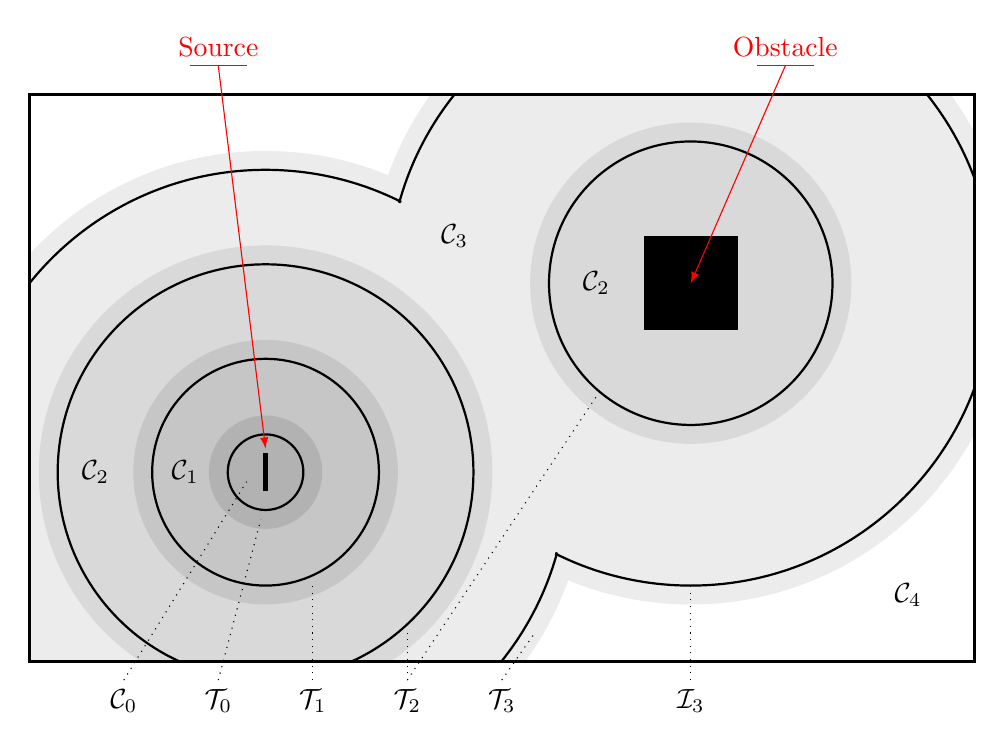
\begin{tikzpicture}[scale=1.2]
		
		\begin{scope}
			\clip (0,0) rectangle (10,6);
			
			% T4
			\draw (9.3,0.7) node {$\mathcal{C}_4$};
			
			% R3
			\fill[gray!15] (7,4) circle (3.4);
			\fill[gray!15] (2.5,2) circle (3.4);

			% T3
			\draw[thick] (7,4) circle (3.2);
			\draw[thick] (2.5,2) circle (3.2);
			\fill[gray!15] (7,4) circle (3.18);
			\fill[gray!15] (2.5,2) circle (3.18);
			\draw (4.5,4.5) node {$\mathcal{C}_3$};

			%---------------------
			% obstacle
			%---------------------
			% R2
			\fill[gray!30] (7,4) circle (1.7);

			% T2
			\draw[thick,fill=gray!30] (7,4) circle (1.5);
			\draw (6,4) node {$\mathcal{C}_2$};
			
			%---------------------
			% source
			%---------------------
			% R2
			\fill[gray!30] (2.5,2) circle (2.4);
			
			% T2
			\draw[thick,fill=gray!30] (2.5,2) circle (2.2);
			\draw (0.7,2) node {$\mathcal{C}_2$};
			
			% R1
			\fill[gray!45] (2.5,2) circle (1.4);
			
			% T1
			\draw[thick,fill=gray!45] (2.5,2) circle (1.2);
			\draw (1.65,2) node {$\mathcal{C}_1$};

			% R0
			\fill[gray!60] (2.5,2) circle (0.6);
						
			% T0
			\draw[thick,fill=gray!60] (2.5,2) circle (0.4);
		\end{scope}
		\draw[very thick] (0,0) rectangle (10,6);

		% T0
		\draw (1,-0.2) node[below] {$\mathcal{C}_0$};
		\draw[dotted] (1,-0.2) -- (2.3,1.9);
	
		% R0
		\draw (2,-0.2) node[below] {$\mathcal{T}_0$};
		\draw[dotted] (2,-0.2) -- (2.45,1.5);
		
		% R1
		\draw (3,-0.2) node[below] {$\mathcal{T}_1$};
		\draw[dotted] (3,-0.2) -- (3,0.8);
		
		% R2
		\draw (4,-0.2) node[below] {$\mathcal{T}_2$};
		\draw[dotted] (4,-0.2) -- (4,0.3);
		\draw[dotted] (4,-0.2) -- (6,2.8);
		
		% R3
		\draw (5,-0.2) node[below] {$\mathcal{T}_3$};
		\draw[dotted] (5,-0.2) -- (5.35,0.3);
		
		% I3
		\draw (7,-0.2) node[below] {$\mathcal{I}_3$};
		\draw[dotted] (7,-0.2) -- (7,0.8);
		
		% Source
		\fill (2.47,1.8) rectangle (2.53,2.2);
		\draw (2,6.3) node[red,above] {Source};
		\draw[-,red] (1.7,6.3) -- (2.3,6.3); 
		\draw[-,red,arrows={-latex}] (2,6.3) -- (2.5,2.25);
		
		% Obstacle
		\fill (6.5,3.5) rectangle (7.5,4.5);
		\draw (8,6.3) node[red,above] {Obstacle};
		\draw[-,red] (7.7,6.3) -- (8.3,6.3); 
		\draw[-,red,arrows={-latex}] (8,6.3) -- (7,4);

		\end{tikzpicture}
	\end{center}
\end{figure}


\subsection{Algorithme}
\label{ssect:lts2_implem_algo}

Avec ces notations, nous pouvons écrire le schéma en temps correspondant
à la figure \ref{img:ader_flux_lrk_ldt}. Ce schéma est composé d'une
boucle principale permettant d'intégrer toutes les mailles sur un pas
de temps complet $\dt^l_{\max}$. Cette boucle est composée de $2^{N_t}$
étapes. Les mailles de la classe $\mathcal{C}_0$ avancent d'un pas de temps
$\dt_{\min}$ à chaque étape. Les mailles de la classe $\mathcal{C}_{N_t}$
n'avancent qu'une seule fois d'un pas de temps $\dt^l_{\max}$ à la dernière
étape. Plus généralement, les mailles de la classe $\mathcal{C}_j$ avancent
$2^{N_t - j}$ fois d'un pas de temps $2^j \dt_{\min}$.

Contrairement au schéma de la figure \ref{img:ader_flux_lrk_ldt},
nous indiçons les itérations de la solution par rapport au pas de 
temps maximal afin que les termes de la suite résultante soient totalement
définis sur le maillage complet.

Ainsi, considérons connue la solution du problème à résoudre
au temps $t = n \dt^l_{\max}$.
A chaque étape $i \in \Range{1}{2^{N_t}}$,
pour tous les $j \in \Range{0}{N_t}$ tels que $2^j$ divise $i$,
avec $k$ l'indice de l'étape courante de la classe $\mathcal{C}_j$ :
\begin{align}
	k \in \EnsN : i = 2^j (k+1) ,
\end{align}
$r$ l'indicateur de décalage temporel de la dernière solution calculée
entre la classe $\mathcal{C}_j$ et les mailles tampon $\mathcal{T}_j$ :
\begin{align}
	r \in \lbrace 0 , 1 \rbrace : k \equiv r \; \lbrack 2 \rbrack ,
\end{align}
$\dt^l_j$ le pas de temps local associé à la classe $\mathcal{C}_j$ :
\begin{align}
	\dt^l_j = 2^j \dt_{\min} = 2^{j-N_t} \dt^l_{\max} = \alpha \dt^l_{\max} ,
\end{align}
$s$ l'indice temporel de la dernière solution intermédiaire calculée :
\begin{align}
	s =
	\begin{cases}
		n + \alpha k & \mathrm{sur} \; \mathcal{C}_j , \\
		n + \alpha (k - r) & \mathrm{sur} \; \mathcal{T}_j ,
	\end{cases}
\end{align}
et $p$ l'indice temporel de la prédiction servant à calculer la solution
intermédiaire suivante :
\begin{align}
	p = n + \alpha \left( k + \frac{1}{2} \right) =
	\begin{cases}
		s + \frac{\alpha}{2} & \mathrm{sur} \; \mathcal{C}_j , \\
		s + \alpha \left( \frac{1}{2} + r \right) & \mathrm{sur} \; \mathcal{T}_j ,
	\end{cases}
\end{align}
%\begin{equation}
%	\begin{aligned}
%		k \in \EnsN : i &= 2^j (k+1) , \\
%		r &\in \lbrace 0 , 1 \rbrace : k \equiv r \; \lbrack 2 \rbrack , \\
%		\alpha &= 2^{j-N_t} , \\
%		\tau &= 2^j \dt_{\min} = \alpha \dt^l_{\max} , \\
%		t &= n \dt^l_{\max} , \\
%		s &= \begin{cases}
%			n + \alpha k & \mathrm{sur} \; \mathcal{C}_j , \\
%			n + \alpha (k - r) & \mathrm{sur} \; \mathcal{T}_j ,
%		\end{cases} \\
%		p &= n + \alpha \left( k + \frac{1}{2} \right) ,
%	\end{aligned}
%\end{equation}
nous avons :
\begin{equation}
	\begin{aligned}
		\V^p &= 
			\W^s + (p-s) \dt^l_{\max}
			\mathcal{G}_l(\W^s , s \dt^l_{\max}) ,
			\; \mathrm{sur} \; \mathcal{C}_j \cup \mathcal{T}_j , \\
		\W^{s + \alpha} &=
			\W^s + \alpha \dt^l_{\max}
			\mathcal{G}(\V^p , p \dt^l_{\max}) ,
			\; \mathrm{sur} \; \mathcal{C}_j ,
		\label{eq:methode_locale}
	\end{aligned}
\end{equation}
avec l'opérateur $\mathcal{G}$ intégrant les flux suivants aux interfaces
de la classe $\mathcal{C}_j$ :
\begin{align}
	\begin{cases}
		\Flux{\V_\L^p}{\V_\R^p}{\n} &
			\mathrm{sur} \; \mathcal{I}_j^{-} , \\
		\frac{1}{2} \left( \Flux{\V_\L^{p-\frac{\alpha}{4}}}{\V_\R^{p-\frac{\alpha}{4}}}{\n} + \Flux{\V_\L^{p+\frac{\alpha}{4}}}{\V_\R^{p+\frac{\alpha}{4}}}{\n} \right) &
			\mathrm{sur} \; \mathcal{I}_{j-1}^{+} , j > 0 ,
	\end{cases}
\end{align}
où $\mathcal{I}_j^{+}$, respectivement $\mathcal{I}_j^{-}$, représente
le côté $\mathcal{T}_j$, respectivement $\mathcal{C}_j$, de l'interface
$\mathcal{I}_j$ dans le cadre du stockage et de l'application des flux
entre deux classes de pas de temps.

Après ces $2^{N_t}$ étapes, toutes les mailles du maillage sont avancées au temps
$n \dt^l_{\max} + 2^{N_t} \dt_{\min} = (n+1) \dt^l_{\max}$.
Le graphe des tâches du schéma couplé GD-LTS$2$ est donné dans la figure \ref{img:graphe_lts2}. Ce graphe représente le calcul d'un pas de
temps $\dt^l_{\max}$ sur $2$ classes de pas de temps.
\\


\begin{figure}[!h]
	\centering
	\caption{
		\label{img:graphe_lts2}
		Graphe des tâches d'un pas de temps $\dt^l_{\max}$ du schéma couplé GD-LTS$2$
		pour $2$ classes de pas de temps.
	}
	\begin{tikzpicture}[
		scale=0.475,
		every node/.style={scale=0.475},
		]
	\node[ellipse,thick,draw,align=center] (debut)
	at (0,0) {Début du grand\\pas de temps};
	
	\node[ellipse,thick,draw,align=center] (debutmin1)
	at (0,-2) {Début du $1^\mathrm{er}$ petit\\pas de temps};
	
	\node[diamond,thick,draw=orange,fill=orange!10,align=center] (prediction11)
	at (-6,-4.5) {Classe $\mathcal{C}_0$\\Prédiction\\$t+0.25$};
	\node[ellipse,thick,draw=blue,fill=blue!10,align=center] (volume11)
	at (-7,-7.5) {Classe $\mathcal{C}_0$\\Terme de volume};
	\node[ellipse,thick,draw=red,fill=red!10,align=center] (flux11)
	at (-6.5,-9.5) {Classe $\mathcal{C}_0$\\Terme de flux};
	\node[ellipse,thick,draw=green,fill=green!10,align=center] (masse11)
	at (-4.5,-11.5) {Classe $\mathcal{C}_0$\\Terme de masse};
	\node[ellipse,thick,draw=gray,fill=gray!10,align=center] (euler11)
	at (-2.5,-13.5) {Classe $\mathcal{C}_0$\\Etape d'Euler};
	
	\node[diamond,thick,draw=orange,fill=orange!10,align=center] (prediction21)
	at (6,-4.5) {Tampon $\mathcal{T}_0$\\Prédiction\\$t+0.25$};
	
	\node[rectangle,thick,draw=red,fill=red!10,align=center] (extract11)
	at (-2,-4.5) {Interface\\Classe $\mathcal{C}_0$\\Extrapolation};
	\node[rectangle,thick,draw=red,fill=red!10,align=center] (apply11)
	at (-2,-8.5) {Interface\\Classe $\mathcal{C}_0$\\Application du flux};
	
	\node[rectangle,thick,draw=red,fill=red!10,align=center] (itfflux1)
	at (0,-6.5) {Interface\\Calcul du flux};
	
	\node[rectangle,thick,draw=red,fill=red!10,align=center] (extract21)
	at (2,-4.5) {Interface\\Tampon $\mathcal{T}_0$\\Extrapolation};
	\node[rectangle,thick,draw=black,align=center] (store21)
	at (2.5,-9.5) {Interface\\Tampon $\mathcal{T}_0$\\Stockage du flux};
	
	\node[ellipse,thick,draw,align=center] (finmin1)
	at (0,-15.5) {Fin du $1^\mathrm{er}$ petit\\pas de temps};
	
	\path[arrows={-latex}] (debut) edge (debutmin1);
	
	\path[arrows={-latex}] (debutmin1) edge[out=180,in=90] (prediction11);
	\path[arrows={-latex}] (debutmin1) edge[out=0,in=90] (prediction21);
	\path[arrows={-latex}] (prediction11) edge (volume11);
	\path[arrows={-latex}] (prediction21) edge[out=270,in=30] (finmin1);
	\path[arrows={-latex}] (volume11) edge (flux11);
	\path[arrows={-latex}] (flux11) edge (masse11);
	\path[arrows={-latex}] (masse11) edge (euler11);
	\path[arrows={-latex}] (euler11) edge (finmin1);
	
	\path[arrows={-latex}] (prediction11) edge[out=0,in=180] (extract11);
	\path[arrows={-latex}] (prediction21) edge[out=180,in=0] (extract21);
	\path[arrows={-latex}] (extract11) edge (itfflux1);
	\path[arrows={-latex}] (extract21) edge (itfflux1);
	\path[arrows={-latex}] (itfflux1) edge (apply11);
	\path[arrows={-latex}] (itfflux1) edge (store21);
	\path[arrows={-latex}] (apply11) edge (masse11);
	\path[arrows={-latex}] (store21) edge (finmin1);
	
	
	\node[ellipse,thick,draw,align=center] (debutmin2)
	at (0,-17.5) {Début du $2^\mathrm{e}$ petit\\pas de temps};
	
	
	\node[diamond,thick,draw=orange,fill=orange!10,align=center] (prediction12)
	at (-9,-20) {Classe $\mathcal{C}_0$\\Prédiction\\$t+0.75$};
	\node[ellipse,thick,draw=blue,fill=blue!10,align=center] (volume12)
	at (-10,-23) {Classe $\mathcal{C}_0$\\Terme de volume};
	\node[ellipse,thick,draw=red,fill=red!10,align=center] (flux12)
	at (-9.5,-25) {Classe $\mathcal{C}_0$\\Terme de flux};
	\node[ellipse,thick,draw=green,fill=green!10,align=center] (masse12)
	at (-7.5,-27) {Classe $\mathcal{C}_0$\\Terme de masse};
	\node[ellipse,thick,draw=gray,fill=gray!10,align=center] (euler12)
	at (-5.5,-29) {Classe $\mathcal{C}_0$\\Etape d'Euler};
	
	\node[diamond,thick,draw=orange,fill=orange!10,align=center] (prediction22)
	at (3,-20) {Tampon $\mathcal{T}_0$\\Prédiction\\$t+0.75$};
	\node[diamond,thick,draw=orange,fill=orange!10,align=center] (prediction23)
	at (3,-24.5) {Tampon $\mathcal{T}_0$\\Prédiction\\$t+0.5$};

	\node[ellipse,thick,draw=blue,fill=blue!10,align=center] (volume21)
	at (3,-28.5) {Classe $\mathcal{T}_0$\\Terme de volume};
	\node[ellipse,thick,draw=red,fill=red!10,align=center] (flux21)
	at (4,-30.5) {Classe $\mathcal{T}_0$\\Terme de flux};
	\node[ellipse,thick,draw=green,fill=green!10,align=center] (masse21)
	at (5,-32.5) {Classe $\mathcal{T}_0$\\Terme de masse};
	\node[ellipse,thick,draw=gray,fill=gray!10,align=center] (euler21)
	at (6,-34.5) {Classe $\mathcal{T}_0$\\Etape d'Euler};

	
	\node[diamond,thick,draw=orange,fill=orange!10,align=center] (prediction31)
	at (14,-24.5) {Classe $\mathcal{C}_1$\\Prédiction\\$t+0.5$};

	\node[ellipse,thick,draw=blue,fill=blue!10,align=center] (volume31)
	at (14,-28.5) {Classe $\mathcal{C}_1$\\Terme de volume};
	\node[ellipse,thick,draw=red,fill=red!10,align=center] (flux31)
	at (13,-30.5) {Classe $\mathcal{C}_1$\\Terme de flux};
	\node[ellipse,thick,draw=green,fill=green!10,align=center] (masse31)
	at (12,-32.5) {Classe $\mathcal{C}_1$\\Terme de masse};
	\node[ellipse,thick,draw=gray,fill=gray!10,align=center] (euler31)
	at (11,-34.5) {Classe $\mathcal{C}_1$\\Etape d'Euler};


	\node[rectangle,thick,draw=red,fill=red!10,align=center] (extract12)
	at (-5,-20) {Interface\\Classe $\mathcal{C}_0$\\Extrapolation};
	\node[rectangle,thick,draw=red,fill=red!10,align=center] (apply12)
	at (-5,-24) {Interface\\Classe $\mathcal{C}_0$\\Application du flux};
	
	\node[rectangle,thick,draw=red,fill=red!10,align=center] (itfflux2)
	at (-3,-22) {Interface\\Calcul du flux};
	
	\node[rectangle,thick,draw=red,fill=red!10,align=center] (extract22)
	at (-1,-20) {Interface\\Tampon $\mathcal{T}_0$\\Extrapolation};
	\node[rectangle,thick,draw=black,align=center] (store22)
	at (-1,-24) {Interface\\Tampon $\mathcal{T}_0$\\Stockage du flux};
	\node[rectangle,thick,draw=red,fill=red!10,align=center] (apply21)
	at (-1,-26.5) {Interface\\Classe $\mathcal{T}_0$\\Application des flux};
	
	
	\node[rectangle,thick,draw=red,fill=red!10,align=center] (extract23)
	at (6.5,-22.5) {Interface\\Classe $\mathcal{T}_0$\\Extrapolation};
	\node[rectangle,thick,draw=red,fill=red!10,align=center] (apply23)
	at (6.5,-26.5) {Interface\\Classe $\mathcal{T}_0$\\Application du flux};
	
	\node[rectangle,thick,draw=red,fill=red!10,align=center] (itfflux3)
	at (8.5,-24.5) {Interface\\Calcul du flux};
	
	\node[rectangle,thick,draw=red,fill=red!10,align=center] (extract31)
	at (10.5,-22.5) {Interface\\Tampon $\mathcal{C}_1$\\Extrapolation};
	\node[rectangle,thick,draw=red,fill=red!10,align=center] (apply31)
	at (10.5,-26.5) {Interface\\Classe $\mathcal{C}_1$\\Application du flux};
	
	
	
	\node[ellipse,thick,draw,align=center] (finmin2)
	at (-1,-32.5) {Fin du $2^\mathrm{e}$ petit\\pas de temps};
	
	\node[ellipse,thick,draw,align=center] (fin)
	at (-3,-34.5) {Fin du grand\\pas de temps};
	
	
	\path[arrows={-latex}] (finmin1) edge (debutmin2);
	\path[arrows={-latex}] (finmin2) edge (fin);
		
	\path[arrows={-latex}] (debutmin2) edge[out=180,in=90] (prediction12);
	\path[arrows={-latex}] (debutmin2) edge[out=0,in=90] (prediction22);
	\path[arrows={-latex}] (debutmin2) edge[out=0,in=90] (prediction31);
	\path[arrows={-latex}] (prediction22) edge (prediction23);
	\path[arrows={-latex}] (prediction12) edge (volume12);
	\path[arrows={-latex}] (prediction23) edge[out=270,in=90] (volume21);
	\path[arrows={-latex}] (prediction31) edge[out=270,in=90] (volume31);
	\path[arrows={-latex}] (volume12) edge (flux12);
	\path[arrows={-latex}] (flux12) edge (masse12);
	\path[arrows={-latex}] (masse12) edge (euler12);
	\path[arrows={-latex}] (euler12) edge (finmin2);

	\path[arrows={-latex}] (volume21) edge (flux21);
	\path[arrows={-latex}] (flux21) edge (masse21);
	\path[arrows={-latex}] (masse21) edge (euler21);
	\path[arrows={-latex}] (euler21) edge[out=180,in=330] (finmin2);
	
	\path[arrows={-latex}] (volume31) edge (flux31);
	\path[arrows={-latex}] (flux31) edge (masse31);
	\path[arrows={-latex}] (masse31) edge (euler31);
	\path[arrows={-latex}] (euler31) edge[out=210,in=320] (finmin2);
	
	\path[arrows={-latex}] (prediction12) edge[out=0,in=180] (extract12);
	\path[arrows={-latex}] (prediction22) edge[out=180,in=0] (extract22);
	\path[arrows={-latex}] (extract12) edge (itfflux2);
	\path[arrows={-latex}] (extract22) edge (itfflux2);
	\path[arrows={-latex}] (extract22) edge (prediction23);
	\path[arrows={-latex}] (itfflux2) edge (apply12);
	\path[arrows={-latex}] (itfflux2) edge (store22);
	\path[arrows={-latex}] (apply12) edge (masse12);
	\path[arrows={-latex}] (store22) edge (apply21);
	\path[arrows={-latex}] (apply21) edge[out=270,in=160] (masse21);

	\path[arrows={-latex}] (prediction23) edge[out=60,in=180] (extract23);
	\path[arrows={-latex}] (prediction31) edge[out=120,in=0] (extract31);
	\path[arrows={-latex}] (extract23) edge (itfflux3);
	\path[arrows={-latex}] (extract31) edge (itfflux3);
	\path[arrows={-latex}] (itfflux3) edge (apply23);
	\path[arrows={-latex}] (itfflux3) edge (apply31);
	\path[arrows={-latex}] (apply23) edge[out=300,in=40] (masse21);
	\path[arrows={-latex}] (apply31) edge[out=240,in=140] (masse31);
	\end{tikzpicture}
\end{figure}




\section{Application à l'équation du transport}
\label{sect:pas de temps local transport}

\subsection{Implémentation en dimension 1}
\label{ssect:lts2 transport implem}

\newcommand{\Vitesse}{u}
Nous appliquons les schémas d'intégration LRK$2$ \eqref{eq:methode_lrk2}
et LTS$2$ \eqref{eq:methode_locale} dans le cas
de l'équation de transport en dimension $1$.
Il s'agit du premier cas d'application qui a permis de vérifier
la validité et la stabilité numérique de ces méthodes.
Ainsi, $\NC = 1$, $\PbEsp = \ItvCC{a}{b} \subset \EnsR$,
$t \in \PbTps \subset \EnsR$,
$\W = w(\x,t)$ et $\A = \Vitesse \in \EnsR$ la vitesse de propagation.
Dans ces conditions, le problème d'évolution s'écrit :
\begin{align}
	\Ptl{t} w + \Vitesse \Ptl{\x} w = 0
	\label{eq:pb_transport_1-d} .
\end{align}

Les nœuds du maillage sont placés à l'aide d'une bijection continue $\sigma$ :
\begin{equation}
	\begin{aligned}
		\sigma : \ItvCC{0}{1} &\to \ItvCC{0}{1} \\
		\x &\mapsto \sigma(\x)
	\end{aligned}
\end{equation}
définie pour contrôler la taille des mailles.
Nous plaçons $\NE + 1$ nœuds $(\Nd{i})_{i \in \Range{0}{\NE}}$
délimitant $\NE$ mailles :
\begin{align}
	\Nd{i} = a + (b - a) \sigma \left( \frac{i}{\NE} \right) ,
\end{align}
d'où :
\begin{align}
	h_i = \Nd{i} - \Nd{i - 1} =
	(b - a) \left( \sigma \left( \frac{i}{\NE} \right) 
		- \sigma \left( \frac{i-1}{\NE} \right) \right) .
\end{align}
Ainsi, lorsque $\sigma(\x) = \x$, les mailles sont homogènes
et le pas de temps est uniforme sur le maillage.
De manière plus générale, si nous prenons pour $\sigma$ une fonction polynomiale
strictement croissante et d'ordre supérieur à $1$,
nous pouvons obtenir un maillage contenant des mailles dilatées sur les
bords, aux voisinages de $a$ et $b$,
et contractées au centre au voisinage de $0$ (figure \ref{img:stretching}).
Pour la réalisation des tests de la méthode, nous nous plaçons
sur l'intervalle $\ItvCC{-1}{1}$.


\begin{figure}[!h]
	\begin{center}
		\caption{
			\label{img:stretching}
			Application de la fonction $\sigma$ 
			sur l'intervalle $\ItvCC{0}{1}$ pour
			$\sigma(\x) = 2 \x^3 - 3 \x^2 + 2 \x$.
			L'intervalle de départ est représenté par l'axe
			horizontal. L'intervalle image est représenté par
			l'axe vertical.
		}
		
		\begin{tikzpicture}[scale=1]
			\begin{axis}[
				axis lines=middle,
				%xlabel=$x$, x label style={at={(axis cs:1.15,0)},anchor=north},
				ylabel=$0$, y label style={at={(axis cs:0,-0.05)},anchor=east},
				xmin=-0.1,xmax=1.1,ymin=-0.1,ymax=1.1,
				xtick={0,1},ytick={0,1},
				%x post scale=1.8,
				%y post scale=2,
				legend style={at={(axis cs:0.9,0.2)},anchor=south west}
				]
				
				\addplot+[
					mark=none,
					color=black,
					domain=0:1
				]
				{2*x^3-3*x^2+2*x};
				\addlegendentry{$\sigma$}
			
				\addplot[
					mark=x,
					only marks,
					mark options={scale=2},
					color=red,
				]
				table {stretching_x.plt};
				\addlegendentry{$\left\lbrace \frac{i}{\NE}, i \in \Range{0}{\NE} \right\rbrace$}
				
				\addplot[
					mark=x,
					only marks,
					mark options={scale=2},
					color=blue,
				]
				table {stretching_y.plt};
				\addlegendentry{$\left\lbrace \sigma \left( \frac{i}{\NE} \right), i \in \Range{0}{\NE} \right\rbrace$}
			\end{axis}
		\end{tikzpicture}
	\end{center}
\end{figure}



Une solution exacte du problème \eqref{eq:pb_transport_1-d} est donnée par :
\begin{align}
w_\mathrm{exact}(\x, t) = \cos(2 \pi (\x - \Vitesse t)) .
\end{align}
Nous simulons donc le déplacement de la solution initiale :
\begin{align}
w_0(\x) = \cos(2 \pi \x) .
\end{align}
Nous effectuons ces simulations dans les cas $\Vitesse = - 1$ et
$\Vitesse = 1$.
\\

\subsection{Prédicteur exact}
\label{ssect:lts2 transport exact pred}


Afin de simplifier l'implémentation de cette application en dimension $1$,
nous choisissons un prédicteur local exact.
Soit $w_\L$ une solution approchée sur la maille $\L$.
Nous pouvons exprimer la valeur de sa dérivée temporelle à partir
de sa décomposition dans la base d'approximation :
\begin{align}
	\Ptl{\x} w_\L (\x,t) \approx 
	\Ptl{\x} \left( \sum_{i=0}^{\Deg} w_{\L,i}(t) \PsiPhy{\L}{i}(\x) \right) =
	\sum_{i=0}^{\Deg} w_{\L,i}(t) \Ptl{\x} \PsiPhy{\L}{i}(\x)
\end{align}
et de la formulation de l'équation du transport \eqref{eq:pb_transport_1-d} :
\begin{align}
	\Ptl{t} w_\L = - \Vitesse \Ptl{\x} w_\L \approx
	- \Vitesse \sum_{i=0}^{\Deg} w_{\L,i}(t) \Ptl{\x} \PsiPhy{\L}{i}(\x) .
\end{align}
Ainsi, en décomposant aussi les dérivées des fonctions de base dans la
base d'approximation, et par orthogonalité des fonctions de base,
nous obtenons le système matriciel suivant :
\begin{align}
	\Ptl{t} \begin{pmatrix}
		w_{\L,0} \\
		\vdots \\
		w_{\L,\Deg}
	\end{pmatrix} + \A
	\begin{pmatrix}
		w_{\L,0} \\
		\vdots \\
		w_{\L,\Deg}
	\end{pmatrix}
	= 0 ,
\end{align}
avec
\begin{align}
	\A = \Vitesse (\Ptl{\x} \PsiPhy{\L}{j} (\GLNPhy{\L}{i}))_{i,j \in \RangeDeg} =
	\Inv{(\TGeo{\L}')} \Vitesse (\Ptl{\xref} \PsiRef{j} (\GLN{i}))_{i,j \in \RangeDeg}
\end{align}
et
\begin{align}
	\TGeo{\L}' = \Jac{\TGeo{\L}} = h_\L.
\end{align}

Le prédicteur local est donné par une exponentielle de matrice, qui est calculable exactement (par exemple
avec un logiciel de calcul formel) :
\begin{align}
	\begin{pmatrix}
		v_{\L,0} \\
		\vdots \\
		v_{\L,\Deg}
	\end{pmatrix}_p =
	\mathrm{exp} ( \dt \A )
	\begin{pmatrix}
		w_{\L,0} \\
		\vdots \\
		w_{\L,\Deg}
	\end{pmatrix}_s .
\end{align}
L'expression de ce prédicteur est donné pour les ordres d'interpolation
$0$, $1$ et $2$ dans le tableau \ref{tab:exact_predictor}.

\begin{figure}[!h]
	\begin{center}
		\caption{
			\label{tab:exact_predictor}
			Expression du prédicteur exact utilisé dans l'implémentation
			du schéma LTS$2$ appliqué à l'équation
			du transport en dimension $1$ pour les ordres d'interpolation
			$0$, $1$ et $2$.
			Nous notons $\lambda = \Inv{(\TGeo{\L}')} \Vitesse \dt$.
		}
		
		\begin{tabular}{|c|c|c|}
			\hline
			$\Deg$ & Solution en $t$ & Prédiction exacte en $t + \dt$ \\
			\hline\hline
			$0$ & $w_{\L,0}$ & $w_{\L,0}$ \\
			\hline
			\multirow{2}{*}{$1$}
			& $w_{\L,0}$ & $(1 + \lambda) w_{\L,0} - \lambda w_{\L,1}$ \\
			& $w_{\L,1}$ & $\lambda w_{\L,0} + (1 - \lambda) w_{\L,1}$ \\
			\hline
			\multirow{3}{*}{$2$}
			& $w_{\L,0}$ & $(1 + \lambda) (1 + 2 \lambda) w_{\L,0} - 4 \lambda (1 + \lambda) w_{\L,1} + \lambda (1 + 2 \lambda) w_{\L,2}$ \\
			& $w_{\L,1}$ & $\lambda (1 + 2 \lambda) w_{\L,0} + (1 - 2 \lambda) (1 + 2 \lambda) w_{\L,1} - \lambda (1 - 2 \lambda) w_{\L,2}$ \\
			& $w_{\L,2}$ & $- \lambda (1 - 2 \lambda) w_{\L,0} + 4 \lambda (1 - \lambda) w_{\L,1} + (1 - \lambda) (1 - 2 \lambda) w_{\L,2}$ \\
			\hline
		\end{tabular}
	\end{center}
\end{figure}


\subsection{Condition de stabilité et convergence}
\label{ssect:lts2 transport stabilite}

Ce cas d'application a expérimentalement été vérifiée stable en temps long
avec un pas de temps uniforme sur tout le maillage 
(schéma LRK$2$ \eqref{eq:methode_lrk2})
pour une condition CFL de type :
\begin{align}
	\dt \le \frac{C(\Deg)}{\Abs{\Vitesse}} \dx
	\label{eq:ader_cfl}
\end{align}
avec $C$ une constante dépendante de l'ordre $\Deg$ dont les valeurs
sont données dans le tableau \ref{tab:ader_trans_cfl}.
Ces valeurs ont été utilisées dans le cas
du schéma LTS$2$ \eqref{eq:methode_locale}
et n'ont généré aucune instabilité.

\begin{figure}[!h]
	\begin{center}
		\caption{
			\label{tab:ader_trans_cfl}
			Valeur de la constante CFL de stabilité $C$ \eqref{eq:ader_cfl}
			utilisée dans l'implémentation du schéma LRK$2$ (et LTS$2$)
			appliqué à l'équation du transport en dimension $1$
			en fonction de l'ordre d'interpolation $\Deg$.
		}
		
		\begin{tabular}{|c|c|}
			\hline
			$\Deg$ & $C(\Deg)$ \\ \hline\hline
			$0$ & $0.56$ \\	\hline
			$1$ & $0.50$ \\	\hline
			$2$ & $0.17$ \\	\hline
			$3$ & $0.08$ \\	\hline
			$4$ & $0.05$ \\	\hline
		\end{tabular}
	\end{center}
\end{figure}



% 1/(2p+1) ? :
% d=0: 1         > 0.9    > 0.56
% d=1: 1/3=0.33  > 0.3    > 0.50
% d=2: 1/5=0.2   > 0.18   > 0.17
% d=3: 1/7=0.143 > 0.129  > 0.08
% d=4: 1/9=0.111 > 0.1    > 0.05

La solution calculée converge vers la solution exacte pour ces conditions
de stabilité. La figure \ref{img:ader_trans_homogene} présente un résultat
dans le cas LRK$2$ avec $\Vitesse = 1$, sur $100$ mailles et
pour l'ordre d'interpolation $\Deg = 2$ jusqu'au temps $\Tmax=1$.
Nous avons choisi la bijection $\sigma(\x) = 2 \x^3 - 3 \x^2 + 2 \x$
représentée dans la figure~\ref{img:stretching} pour ce résultat,
avec un pas de temps homogène sur tout le maillage.


\begin{figure}[!h]
	\begin{center}
		\caption{
			\label{img:ader_trans_homogene}
			Solution calculée $w_\mathrm{calc}$ et solution exacte
			$w_\mathrm{exact}$ de l'équation du transport en dimension $1$
			dans le cas du schéma LRK$2$ (pas de temps homogène) avec
			$\Vitesse = 1$, $\NE = 100$, $\Deg = 2$ et $\Tmax=1$.
		}
		
		\begin{tikzpicture}[scale=1]
			\begin{axis}[
				%axis lines=middle,
				%xlabel=$\x$, x label style={at={(axis cs:1.15,0)},anchor=north},
				%ylabel=$w(\x,\Tmax)$, y label style={at={(axis cs:0,-0.05)},anchor=east},
				%xmin=-1.1,xmax=1.1,
				ymin=-1.2,ymax=1.7,
				xtick={-1,-0.5,0,0.5,1},
				%ytick={-1,-0.5,0,0.5,1},
				x post scale=1.5,
				%y post scale=2,
				%legend style={at={(axis cs:0.9,0.2)},anchor=south west}
				]
				
				\addplot+[
				mark=none,
				%color=black,
				]
				table {ader_trans_homogene_exact.plt};
				\addlegendentry{$w_\mathrm{exact}(\x,\Tmax)$}
				
				\addplot[
				mark=x,
				only marks,
				%mark options={scale=2},
				color=red,
				]
				table {ader_trans_homogene_calc.plt};
				\addlegendentry{$w_\mathrm{calc}(\x,\Tmax)$}
			\end{axis}
		\end{tikzpicture}
	\end{center}
\end{figure}



Les courbes de convergence du schéma LRK$2$ sont données
dans la figure~\ref{img:ader_trans_cv}. Nous pouvons constater
que cette méthode est généralement d'ordre $2$ en temps, tout comme
le schéma RK$2$.
Elle est d'ordre $1$ en temps uniquement lorsque l'ordre d'interpolation
spatiale choisi est $0$.

\begin{remark} \label{rq:cv_temporelle}
	Les résultats de convergence présentés dans les figures 
	\ref{img:ader_trans_cv} et \ref{img:ader_trans_cv_local}
	sont ceux du schéma en temps théoriquement d'ordre $2$.
	Pour constater l'ordre de convergence de la méthode
	d'intégration spatiale, le coefficient CFL devrait être
	choisi très petit afin de minimiser l'erreur induite
	par l'intégration temporelle.
\end{remark}


\begin{figure}[!h]
	\begin{center}
		\caption{
			\label{img:ader_trans_cv}
			Convergence du schéma LRK$2$ (pas de temps homogène)
			appliqué à l'équation du transport en dimension $1$ avec
			$\Vitesse = 1$ et $\Tmax=1$.
			Les points correspondent à l'application de la méthode
			pour les premiers termes ($i \in \Range{0}{3}$)
			de la suite $100 \cdot 2^i$ en nombre de mailles.
		}
		
		\begin{tikzpicture}[scale=1]
			\begin{axis}[
			%axis lines=middle,
			xlabel=$\log\left(\min\limits_{\L}
			h_\L\right)$, %x label style={at={(axis cs:1.15,0)},anchor=north},
			ylabel=$\log\left(\Norm{w_\mathrm{exact} - w_\mathrm{calc}}_{\mathrm{L}^2}\right)$, %y label style={at={(axis cs:0,-0.05)},anchor=east},
			xmin=-7.2,xmax=-3.8,ymin=-17,ymax=2,
			xtick={-7,-6.5,-6,-5.5,-5,-4.5,-4},%ytick={0,1},
			x post scale=1.5,
			%y post scale=2,
			%legend style={at={(axis cs:0.9,0.2)},anchor=south west}
			]
			
			\addplot+[color=blue,mark=x,] plot coordinates {
(-4.60477,	-1.823117)
(-5.298217,	-2.466994)
(-5.99144,	-3.134661)
(-6.684605,	-3.814834)				
			};
			\addlegendentry{$\Deg = 0$}
			
			\addplot+[color=red,mark=x,] plot coordinates {
(-4.60477,	-4.267916)
(-5.298217,	-5.651476)
(-5.99144,	-7.03702)
(-6.684605,	-8.422986)
			};
			\addlegendentry{$\Deg = 1$}
			
			\addplot+[color=green,mark=x,] plot coordinates {
(-4.60477,	-8.890147)
(-5.298217,	-10.51677)
(-5.99144,	-11.984864)
(-6.684605,	-13.392499)
			};
			\addlegendentry{$\Deg = 2$}
			
			\addplot+[color=yellow,mark=x,] plot coordinates {
(-4.60477,	-10.78446)
(-5.298217,	-12.150812)
(-5.99144,	-13.528604)
(-6.684605,	-14.912975)
			};
			\addlegendentry{$\Deg = 3$}
			
			\addplot+[color=pink,mark=x,] plot coordinates {
(-4.60477,	-11.717318)
(-5.298217,	-13.091391)
(-5.99144,	-14.479932)
(-6.684605,	-15.901417)
			};
			\addlegendentry{$\Deg = 4$}
			\end{axis}
		\end{tikzpicture}
	\end{center}
\end{figure}

% Pentes des courbes de CV
% d=0
%0.9285165269
%0.963134518
%0.9812569879
%
% d=1
%1.9951921344
%1.9986988314
%1.9994748725
%
% d=2
%2.3457063049
%2.1177802814
%2.0307358277
%
% d=3
%1.9703769719
%1.9875162826
%1.9971738331
%
% d=4
%1.9815112042
%2.0030221155
%2.0507166403

Dans le cas de l'application du schéma LTS$2$, la solution calculée converge
aussi vers la solution exacte, dans les mêmes conditions que pour le
résultat LRK$2$ de la figure \ref{img:ader_trans_homogene}, à savoir
$\Vitesse = 1$, $\NE = 100$, $\Deg = 2$ et $\Tmax=1$.
Le critère de stabilité $C(2) = 0.17$ donné dans le tableau
\ref{tab:ader_trans_cfl} est encore vérifié dans ce cas.
Nous avons là aussi choisi la bijection $\sigma(\x) = 2 \x^3 - 3 \x^2 + 2 \x$
représentée dans la figure~\ref{img:stretching}, mais cette fois
sans imposer de pas de temps homogène.
Le calcul a donc été effectué avec $2$ classes de pas de temps.
Ce résultat est présenté dans la figure~\ref{img:ader_trans_local}.
Les classes de pas de temps
des mailles y sont aussi représentées par rapport à l'axe de droite.

\begin{figure}[!h]
	\begin{center}
		\caption{
			\label{img:ader_trans_local}
			Solution calculée $w_\mathrm{calc}$ et solution exacte
			$w_\mathrm{exact}$ de l'équation du transport en dimension $1$
			dans le cas du schéma LTS$2$ (pas de temps local)
			pour $\Vitesse = 1$, $\NE = 100$, $\Deg = 2$, $\Tmax=1$
			et $2$ classes de pas de temps.
			La valeur de la solution est donnée par l'axe de gauche.
			La classe de pas de temps est donnée par l'axe de droite.
			Agrandissement de la solution au voisinage d'une interface
			située entre les classes de pas de temps.
		}
		
		\begin{tikzpicture}[scale=1]
		\begin{axis}[
		hide x axis,
		x post scale=1.5,
		axis y line*=right,
		ymin=-0.2,ymax=2.7,
		ytick={0,1},
		]

		\addplot+[
		mark=none,
		color=green,
		]
		table {ader_trans_local_levels.plt}; \label{plot_3}
		%\addlegendentry{$\lbrace i : \x \in \L \in \mathcal{C}_i \rbrace$}
		
		\end{axis}

		\begin{axis}[
		%axis lines=middle,
		%xlabel=$\x$, x label style={at={(axis cs:1.15,0)},anchor=north},
		%ylabel=$w(\x,\Tmax)$, y label style={at={(axis cs:0,-0.05)},anchor=east},
		%xmin=-1.1,xmax=1.1,
		ymin=-1.2,ymax=1.7,
		xtick={-1,-0.5,0,0.5,1},%ytick={0,1},
		x post scale=1.5,
		axis y line*=left,
		%y post scale=2,
		%legend style={at={(axis cs:0.9,0.2)},anchor=south west}
		]
		
		\addplot+[
		mark=none,
		%color=black,
		]
		table {ader_trans_local_exact.plt};
		\addlegendentry{$w_\mathrm{exact}(\x,\Tmax)$}
		
		\addplot[
		mark=x,
		only marks,
		%mark options={scale=2},
		color=red,
		]
		table {ader_trans_local_calc.plt};
		\addlegendentry{$w_\mathrm{calc}(\x,\Tmax)$}
		
		\addlegendimage{/pgfplots/refstyle=plot_3}\addlegendentry{$\lbrace i : \x \in \L \in \mathcal{C}_i \rbrace$}
				
		\end{axis}
		
		\end{tikzpicture}
		\\
		\begin{tikzpicture}[scale=1]
		\begin{axis}[
		hide x axis,
		x post scale=1.5,
		axis y line*=right,
		xmin=-0.51,xmax=-0.24,
		ymin=-0.1,ymax=1.1,
		ytick={0,1},
		]
		
		\addplot+[
		mark=none,
		color=green,
		]
		table {ader_trans_local_levels.plt};
		
		\end{axis}
		
		\begin{axis}[
		xmin=-0.51,xmax=-0.24,
		ymin=-1.1,ymax=0.1,
		xtick={-0.5,-0.45,-0.4,-0.35,-0.3,-0.25},
		x post scale=1.5,
		axis y line*=left,
		]
		
		\addplot+[
		mark=none,
		%color=black,
		]
		table {ader_trans_local_exact.plt};
		
		\addplot[
		mark=x,
		only marks,
		%mark options={scale=2},
		color=red,
		]
		table {ader_trans_local_calc.plt};
		
		\end{axis}
		
		\end{tikzpicture}
	\end{center}
\end{figure}



Les courbes de convergence du schéma LTS$2$ sont données
dans la figure~\ref{img:ader_trans_cv_local}. Nous pouvons constater
que cette méthode est aussi d'ordre $2$ en temps, tout comme
les schémas RK$2$ et LRK$2$.
Là aussi, ce schéma est d'ordre $1$ en temps uniquement lorsque l'ordre
d'interpolation spatiale choisi est $0$.


\begin{figure}[!h]
	\begin{center}
		\caption{
			\label{img:ader_trans_cv_local}
			Convergence du schéma LTS$2$ (pas de temps local)
			appliqué à l'équation du transport en dimension $1$, pour
			$\Vitesse = 1$ et $\Tmax=1$.
			Les points correspondent à l'application de la méthode
			pour les premiers termes ($i \in \Range{0}{3}$)
			de la suite $100 \cdot 2^i$ en nombre de mailles.
			Les courbes en pointillés sont, à titre de comparaison,
			celles obtenues
			avec un pas de temps homogène (figure
			\ref{img:ader_trans_cv}).
			Les résultats de convergence pour LRK$2$ avec $\Deg=3$
			sont masqués par les résultats pour LTS$2$ avec $\Deg=4$.
		}
		
		\begin{tikzpicture}[scale=1]
		\begin{axis}[
		%axis lines=middle,
		xlabel=$\log\left(\min\limits_{\L}
		h_\L\right)$, %x label style={at={(axis cs:1.15,0)},anchor=north},
		ylabel=$\log\left(\Norm{w_\mathrm{exact} - w_\mathrm{calc}}_{\mathrm{L}^2}\right)$, %y label style={at={(axis cs:0,-0.05)},anchor=east},
		xmin=-7.2,xmax=-3.8,ymin=-17,ymax=2,
		xtick={-7,-6.5,-6,-5.5,-5,-4.5,-4},%ytick={0,1},
		x post scale=1.5,
		%y post scale=2,
		%legend style={at={(axis cs:0.9,0.2)},anchor=south west}
		]
		
		% lrk2
		\addplot+[color=blue,mark=x,dashed,forget plot,mark=none,] plot coordinates {
			(-4.60477,	-1.823117)
			(-5.298217,	-2.466994)
			(-5.99144,	-3.134661)
			(-6.684605,	-3.814834)				
		};
		
		\addplot+[color=red,mark=x,dashed,forget plot,mark=none,] plot coordinates {
			(-4.60477,	-4.267916)
			(-5.298217,	-5.651476)
			(-5.99144,	-7.03702)
			(-6.684605,	-8.422986)
		};
		
		\addplot+[color=green,mark=x,dashed,forget plot,mark=none,] plot coordinates {
			(-4.60477,	-8.890147)
			(-5.298217,	-10.51677)
			(-5.99144,	-11.984864)
			(-6.684605,	-13.392499)
		};
		
		\addplot+[color=yellow,mark=x,dashed,forget plot,mark=none,] plot coordinates {
			(-4.60477,	-10.78446)
			(-5.298217,	-12.150812)
			(-5.99144,	-13.528604)
			(-6.684605,	-14.912975)
		};
		
		\addplot+[color=pink,mark=x,dashed,forget plot,mark=none,] plot coordinates {
			(-4.60477,	-11.717318)
			(-5.298217,	-13.091391)
			(-5.99144,	-14.479932)
			(-6.684605,	-15.901417)
		};


		% dt local
		\addplot+[color=blue,mark=x,] plot coordinates {
			(-4.60477,	-2.547185)
			(-5.298217,	-3.222568)
			(-5.99144,	-3.904866)
			(-6.684605,	-4.593456)				
		};
		\addlegendentry{$\Deg = 0$}
		
		\addplot+[color=red,mark=x,] plot coordinates {
			(-4.60477,	-4.805638)
			(-5.298217,	-6.191844)
			(-5.99144,	-7.577977)
			(-6.684605,	-8.964038)
		};
		\addlegendentry{$\Deg = 1$}
		
		\addplot+[color=green,mark=x,] plot coordinates {
			(-4.60477,	-8.233455)
			(-5.298217,	-9.665441)
			(-5.99144,	-11.062695)
			(-6.684605,	-12.451157)
		};
		\addlegendentry{$\Deg = 2$}
		
		\addplot+[color=yellow,mark=x,] plot coordinates {
			(-4.60477,	-9.811962)
			(-5.298217,	-11.190979)
			(-5.99144,	-12.574252)
			(-6.684605,	-13.96005)
		};
		\addlegendentry{$\Deg = 3$}

		\addplot+[color=pink,mark=x,] plot coordinates {
			(-4.60477,	-10.745377)
			(-5.298217,	-12.129452)
			(-5.99144,	-13.517749)
			(-6.684605,	-14.917156)
		};
		\addlegendentry{$\Deg = 4$}
		\end{axis}
		\end{tikzpicture}
	\end{center}
\end{figure}

% Pentes des courbes de CV
% d=0
%0.9739504245
%0.9842402805
%0.9933998399
%
% d=1
%1.999007855
%1.9995484858
%1.999611925
%
% d=2
%2.065025878
%2.0155909426
%2.0030757468
%
% d=3
%1.9886408046
%1.9954228293
%1.999232506
%
% d=4
%1.9959348011
%2.0026701364
%2.0188656381


Ces résultats démontrent la capacité de cette méthode à produire des
solutions de bonne qualité. Nous avons aussi la preuve que notre
méthode d'application des flux sur les mailles tampon est conservative.
Dans notre cas d'étude, la solution se déplace dans un sens, mais
les interfaces entre les classes de pas de temps sont définies dans
les deux sens de la direction étudiée.
Nous avons présenté des résultats dans le cas $\Vitesse=1$. Les résultats
dans le cas $\Vitesse=-1$ sont identiques, hormis le sens de déplacement
opposé.

\begin{remark}
	Dans notre implémentation, nous avons choisi d'utiliser un prédicteur exact.
	La propriété de convergence de la méthode dépend de la qualité du prédicteur.
	Dans la section suivante, pour l'application aux équations de Maxwell
	en dimension $3$, nous utiliserons l'opérateur
	$\mathcal{G}_l$ dans les phases de prédiction.	
\end{remark}



\subsection{Performances}
\label{ssect:lts2 transport perfs}

\begin{remark}
	Le programme qui nous a servi à évaluer les performances de
	cette méthode appliquée à l'équation du transport en dimension $1$
	a été codé en C, sans optimisation particulière.
\end{remark}

Maintenant que la convergence et la stabilité de la méthode sont assurés,
nous pouvons évaluer le gain de performance apporté par celle-ci.
Intuitivement, une telle méthode devrait produire un temps de calcul
inférieur de la forme :
\begin{align}
	T_\mathrm{s}(\mathrm{LTS2},\Mesh) \ge
	T_\mathrm{i}(\mathrm{LTS2},\Mesh) = \frac{T_\mathrm{s}(\mathrm{LRK2},\Mesh)}{\#\Mesh}
		\sum_{i=0}^{N_t} \frac{1}{2^i} \#\mathcal{C}_i ,
	\label{eq:ader_t_simu_locale}
\end{align}
où $T_\mathrm{s}$ représente le temps de calcul d'une simulation pour une méthode
donnée sur un ensemble de mailles,
$T_\mathrm{i}$ représente le temps de calcul idéal (théorique)
d'une méthode
et $\#\lbrack.\rbrack$ représente le cardinal d'un ensemble.

En effet, au cours d'une étape du schéma LTS$2$,
chaque classe de pas de temps $\mathcal{C}_i$ n'effectue que
$2^{N_t - i}$ étapes de prédiction et mise-à-jour dans le calcul
d'un pas de temps $\dt_{\max}^l$ qui se décompose en $2^{N_t}$ pas
de temps $\dt_{\min}$. Le temps de calcul pour une classe de pas de temps
est donc donné par la proportion d'étapes effectuées :
\begin{align}
	\frac{2^{N_t - i}}{2^{N_t}} = \frac{1}{2^i}
\end{align}
multiplié par le temps de calcul engendré par les mailles
de cette classe :
\begin{align}
	T_\mathrm{s}(\mathrm{LTS2},\mathcal{C}_i) \approx 
		\frac{1}{2^i} \frac{T_\mathrm{s}(\mathrm{LRK2},\Mesh)}{\#\Mesh} \#\mathcal{C}_i .
\end{align}

La formule \eqref{eq:ader_t_simu_locale} nous donne une expression du
temps de simulation idéal en appliquant le schéma LTS$2$.
Cependant, cette formule ne tient pas compte des mailles tampon qui nécessitent
plus de calculs que leurs mailles voisines.

Nous donnons des résultats de performance en fonction de la taille des classes
de pas de temps dans le tableau \ref{tab:ader_trans_perf}.
Nous nous contentons de $2$ classes de pas de temps et choisissons des
bijections de la forme $\sigma(\x) = \alpha \x^3 + (1 - \alpha) \x$.
Ainsi, nous imposons les classes de pas de temps :
\begin{subequations}
	\begin{align}
		{\mathcal{C}'}_0 &= \mathcal{C}_0 ,
		\\
		{\mathcal{C}'}_1 &= \bigcup_{i \in \Range{1}{N_t}} \mathcal{C}_i .
	\end{align}
\end{subequations}


\begin{figure}[!h]
	\begin{center}
		\caption{
			\label{tab:ader_trans_perf}
			Facteurs de gain de temps mesurés (et idéal) du schéma LTS$2$
			appliqué à l'équation du transport en dimension $1$
			par rapport au schéma LRK$2$ pour différentes
			tailles de $2$ classes de pas de temps
			et différents ordres d'interpolation $\Deg$.
			Le paramètre $\alpha$ intervient dans l'expression de la
			bijection $\sigma(\x) = \alpha \x^3 + (1 - \alpha) \x$.
		}
		
		\begin{tabular}{|c|c|c|c|c|c|c|}
			\hline
			$\alpha$ & $\#{\mathcal{C}'}_0$ & $\#{\mathcal{C}'}_1$ & $\Deg = 1$ & $\Deg = 2$ & $\Deg = 3$ & Idéal \\ \hline\hline
			$0.5$ & 579 & 421 & 0.99 & 0.90 & 0.80 & 0.7895 \\	\hline
			% d=1 lrk2: 1938	lts2: 1910
			% d=2 lrk2: 9764	lts2: 8797
			% d=3 lrk2: 5721	lts2: 4564
			$0.7$ & 380 & 620 & 0.87 & 0.78 & 0.73 & 0.69 \\	\hline
			% d=1 lrk2: 1938	lts2: 1684
			% d=2 lrk2: 9835	lts2: 7708
			% d=3 lrk2: 5478	lts2: 3980
			$0.9$ & 194 & 806 & 0.73 & 0.67 & 0.64 & 0.597 \\	\hline
			% d=1 lrk2: 1982	lts2: 1456
			% d=2 lrk2: 9917	lts2: 6684
			% d=3 lrk2: 5465	lts2: 3480
			$0.99$ & 60 & 940 & 0.66 & 0.61 & 0.56 & 0.53 \\	\hline
			% d=1 lrk2: 1943	lts2: 1292
			% d=2 lrk2: 9694	lts2: 5940
			% d=3 lrk2: 5518	lts2: 3094
			$0.999$ & 20 & 980 & 0.63 & 0.59 & 0.54 & 0.51 \\	\hline
			% d=1 lrk2: 1957	lts2: 1241
			% d=2 lrk2: 9701	lts2: 5736
			% d=3 lrk2: 5461	lts2: 2973
			$1$ & 3 & 997 & 0.63 & 0.58 & 0.53 & 0.5015 \\	\hline
			% d=1 lrk2: 1931	lts2: 1222
			% d=2 lrk2: 9706	lts2: 5620
			% d=3 lrk2: 5492	lts2: 2924
		\end{tabular}
	\end{center}
\end{figure}

Nous constatons que le gain de temps résultant de l'utilisation du schéma LTS$2$
est principalement lié au nombre de mailles présentes dans la classe
de pas de temps $\mathcal{C}_0$.
Moins il y a de mailles dans cette classe, plus le gain de temps est conséquent.
Ce résultat est logique puisque la majeure partie des calculs est effectuée
dans cette classe.
Idéalement, le temps LTS$2$ est la moitié du temps LRK$2$ lorsque
le nombre de mailles dans la classe $\mathcal{C}_0$ passe à $0$.
Toutes les mailles sont alors de classe ${\mathcal{C}'}_1$ et la
résolution s'effectue globalement avec le pas de temps $2 \dt_{\min}$.

Cette méthode est aussi plus efficace en ordre d'interpolation spatiale élevé.
Bien qu'en dimension $1$ et faible ordre d'interpolation spatiale,
ce surcoût ne représente que peu de calculs contrairement à une méthode
en dimension $3$ avec un ordre d'interpolation élevé.
Ce phénomène s'explique par le fait que le surcoût de calculs engendré
par la structure du programme et les mailles tampon sont compensés par la
complexité globale des calculs lorsque l'ordre augmente.

Enfin, pour les cas en ordre spatial $3$ présentés dans le tableau
\ref{tab:ader_trans_perf}, les performances sont proches de celles
données théoriquement par la formule du temps idéal \eqref{eq:ader_t_simu_locale}.


\begin{figure}[!h]
	\begin{center}
		\caption{
			\label{tab:ader_trans_perf_many_classes}
			Facteurs de gain de temps mesurés (et idéal) du schéma LTS$2$
			appliqué à l'équation du transport en dimension $1$
			par rapport au schéma LRK$2$ pour différentes
			tailles de classes de pas de temps
			et différents ordres d'interpolation $\Deg$.
			Le paramètre $\alpha$ intervient dans l'expression de la
			bijection $\sigma(\x) = \alpha \x^3 + (1 - \alpha) \x$.
		}
		
		\begin{tabular}{|c|c|c|c|c|c|}
			\hline
			$\alpha$ & $(\#\mathcal{C}_0, \#\mathcal{C}_1, \ldots)$ & $\Deg = 1$ & $\Deg = 2$ & $\Deg = 3$ & Idéal \\ \hline\hline
			$0.5$ & $(579,421)$ & 0.99 & 0.90 & 0.80 & $\approx$ 0.79 \\	\hline
			% d=1 lrk2: 1938	lts2: 1910
			% d=2 lrk2: 9764	lts2: 8797
			% d=3 lrk2: 5721	lts2: 4564
			$0.7$ & $(380,277,343)$ & 0.75 & 0.68 & 0.64 & $\approx$ 0.60 \\	\hline
			% d=1 lrk2: 1938	lts2: 1453
			% d=2 lrk2: 9835	lts2: 6726
			% d=3 lrk2: 5478	lts2: 3522
			$0.9$ & $(194,141,176,236,253)$ & 0.46 & 0.41 & 0.39 & $\approx$ 0.35 \\	\hline
			% d=1 lrk2: 1982	lts2: 903
			% d=2 lrk2: 9917	lts2: 4022
			% d=3 lrk2: 5465	lts2: 2117
			$0.99$ & $(60,43,53,71,98,138,193,273,71)$ & 0.17 & 0.14 & 0.13 & $\approx$ 0.12 \\	\hline
			% d=1 lrk2: 19189	lts2: 3180
			% d=2 lrk2: 97845	lts2: 13917
			% d=3 lrk2: 54631	lts2: 7181
		\end{tabular}
	\end{center}
\end{figure}

Dans le tableau \ref{tab:ader_trans_perf_many_classes}, les résultats
de performances sont présentés pour les mêmes simulations que celles
présentées dans le tableau \ref{tab:ader_trans_perf}.
Pour cette seconde salve de résultats, nous n'avons pas forcé le nombre
de classes de pas de temps à $2$. Celles-ci sont en nombre croissant en
fonction du paramètre $\alpha$ de la bijection $\sigma$ utilisée.

Nous constatons que plus le nombre de classes augmente, plus le temps
idéal diminue et plus le gain de temps augmente.
Ainsi, à l'ordre spatial $1$, avec les $9$ classes de pas de temps ($N_t=8$)
du cas $\alpha = 0.99$, le facteur d'accélération est d'approximativement $6$.
Ce facteur d'accélération passe à $7.6$ pour l'ordre spatial $3$.

D'importantes accélérations sont réalisables avec cette méthode,
dans les cas où la géométrie est bien adaptée.
Son efficacité est directement liée à l'hétérogénéité de la taille des mailles.
Lorsque les tailles des mailles sont homogènes, aucun gain ne sera constaté.
Au contraire, plus le facteur d'échelle entre les mailles est important
et moins il y a de petites mailles, meilleure sera l'accélération.
\\

Nous présentons des résultats de l'application
de cette méthode aux équations de Maxwell en dimension $3$
dans la section \ref{ssect:tete_simplifiee_dt_local}.
\\


\section*{Conclusion}


Dans ce chapitre, nous avons présenté
une variante locale de la méthode GD décrite au chapitre
\ref{chap:generalites}. Cet opérateur d'intégration local
permet d'alléger les calculs de flux et de découpler l'avancée en
temps des mailles. Notons toutefois que cet opérateur local
n'est à utiliser qu'en phase de prédiction (calcul des points
d'intégration temporels), une mise-à-jour
globale est nécessaire à chaque étape du calcul
dans le but d'assurer la stabilité du schéma.

Cet opérateur local nous a permis de décrire deux schémas temporels.
Le schéma LRK$2$ qui est une implémentation à prédiction locale
du schéma RK$2$ (section \ref{ssect:rk}). Ce schéma utilise
un pas de temps homogène sur tout le maillage.
Il a expérimentalement été démontré convergeant et stable.
Nous verrons cependant dans la section \ref{ssect:tete_simplifiee_lrk2}
que ce schéma est moins intéressant en temps de calcul que le schéma RK$2$
car ce dernier admet un coefficient CFL de stabilité
plus grand.

Nous avons aussi présenté le schéma LTS$2$ pour lequel le pas de
temps est local à chaque maille.
Pour ce schéma, les mailles sont réparties en classes de pas de temps :
sous-ensembles de mailles sur lesquels le pas de temps est homogène.
Le schéma LRK$2$ est alors localement appliqué sur ces classes
avec une intégration temporelle spéficique aux interfaces entre les classes.
Ce second schéma a lui aussi été expérimentalement démontré convergeant et stable.
Les accélérations obtenues à l'aide de cette méthode sont
très proches de l'accélération théorique en dimension $1$.
Nous constaterons aussi une accélération des calculs
en dimension $3$ dans la section \ref{ssect:tete_simplifiee_dt_local}.
Ce schéma LTS$2$ permet de réduire
considérablement le temps de simulation en divisant la quantité
de calculs lorsque la géométrie est composée de mailles de tailles très hétérogènes.
\\


Dans le chapitre suivant, nous allons présenter les résultats
de l'exécution du solveur GD \texttt{schnaps} sur architecture hybride
(composition de CPU et/ou GPU hétérogènes).
Pour cela nous avons utilisé (entre autres) la bibliothèque StarPU
développée à l'INRIA de Bordeaux
\cite{augonnet2011starpu,augonnet2012starpu}.
Des expérimentations d'équilibrage automatique de la charge
de calcul entre les différents supports d'exécution
ont aussi été effectuées à l'aide de la bibliothèque de
partitionnement \texttt{metis} \cite{Karypis:1998:FHQ:305219.305248}.


